\subsection{Comparison of Prediction Methods}

EG01-EG23, EG01-EG24, EG01-EG29, and EG01-EG30 transition scenarios
are set up in \Cyclus using \deploy. 
EG01-23 and EG01-29 transition scenario simulations have a constant 
power demand, while EG01-24 and EG01-30 have a linearly increasing
power demand. 
We identified the most effective d3ploy prediction method 
for each scenario by comparing the results of using each 
prediction method in each scenario. 
Similar to the simple transition scenario, these transition scenario 
simulations begin with an initial fleet of \glspl{LWR} 
that start progressively decommissioning at the 80-year mark, 
after which \deploy deploys \glspl{SFR} and \gls{MOX} \glspl{LWR} to meet 
the power demand. 
Figure \ref{fig:eg2329}
shows the setup of facilities and mass flows for 
EG01-23 and EG01-29 in \Cyclus. 
In EG01-23 and EG01-29, recycled plutonium from LWR spent fuel 
produces  \gls{SFR} fuel. 
EG01-24 and EG01-30 are similar to EG01-23 and EG01-29, respectively, 
with the exception that all transuranic elements are recycled.

\begin{figure}[]
	\centering
	\begin{subfigure}[t]{\textwidth}
		\centering
		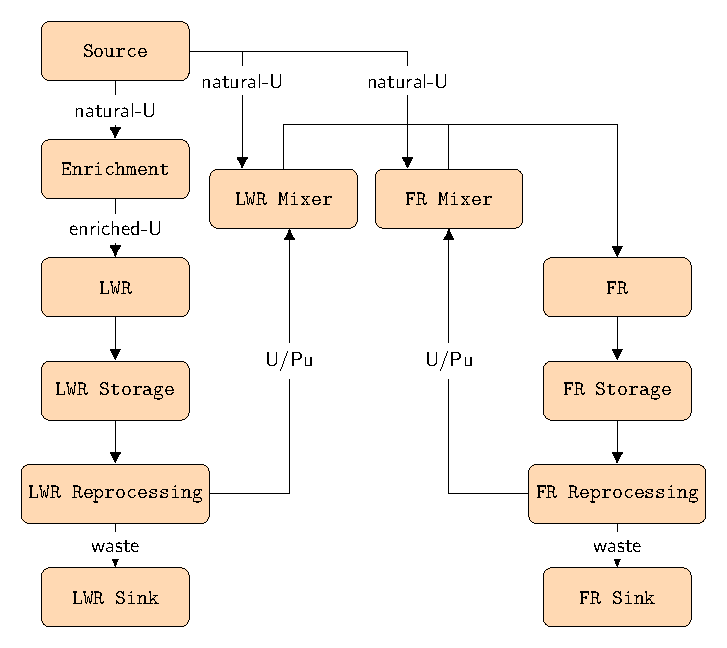
\includegraphics[width=0.65\linewidth]{23flow.pdf} 
		\caption{EG01-EG23.}
		\label{fig:23flow}
	\end{subfigure}
	\vspace{1cm}
	\begin{subfigure}[t]{\textwidth}
		\centering
		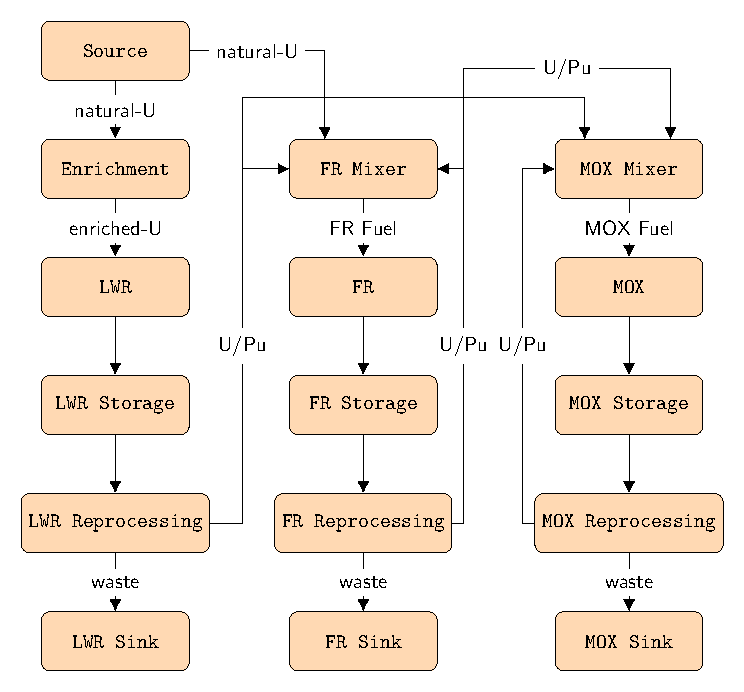
\includegraphics[width=0.65\linewidth]{29flow.pdf} 
		\caption{EG01-EG29.}
		\label{fig:29flow}
	\end{subfigure}
	\hfill
	\caption{Facility and mass flow of the transition scenarios EG01-EG23 and EG01-EG29 in \Cyclus.}
	\label{fig:eg2329}
\end{figure}

In Figure \ref{fig:eg23under}, crosses represent the time steps in which there exists
undersupply or under-capacity of each commodity for the constant power 
EG01-23 transition scenario.
The size of the crosses are proportional to the undersupply value. 
Table \ref{tab:all-power} shows the number of time steps with power 
undersupply for constant power EG01-EG23 and EG01-29, 
linearly increasing power EG01-24 and EG01-30 transition scenarios. 
Figure \ref{fig:eg23under} demonstrates that the \texttt{POLY} and 
\texttt{FFT} methods perform the best for the EG01-23 transition scenario,
with the least number of points on the plot, 
indicating they have the fewest number of time 
steps with undersupply and under-capacity of commodities. 
Table \ref{tab:all-power} shows that the \texttt{POLY} method performs slightly 
better at minimizing undersupply of power than the \texttt{FFT} method, 
with only 6 power undersupplied time steps.
We conducted a similar analysis for the constant power EG01-29 scenario,
and as seen in Table \ref{tab:all-power}, the \texttt{POLY} prediction method 
also performed best for minimizing undersupply of power.  

In Figure \ref{fig:eg24under}, crosses represent the time steps in which 
there exists undersupply or under-capacity of each commodity for a linearly 
increasing power EG01-24 transition scenario.
Figure \ref{fig:eg24under} demonstrates that the \texttt{FFT} method 
performs the best at minimizing the undersupply of all commodities.
We conducted a similar analysis for the constant power EG01-30 scenario, and 
as seen in Table \ref{tab:all-power}, the \texttt{FFT} prediction method also performed 
best for minimizing undersupply of power. 

\begin{figure}[]
	\centering
	\begin{subfigure}[t]{1.2\textwidth}
		\centering
		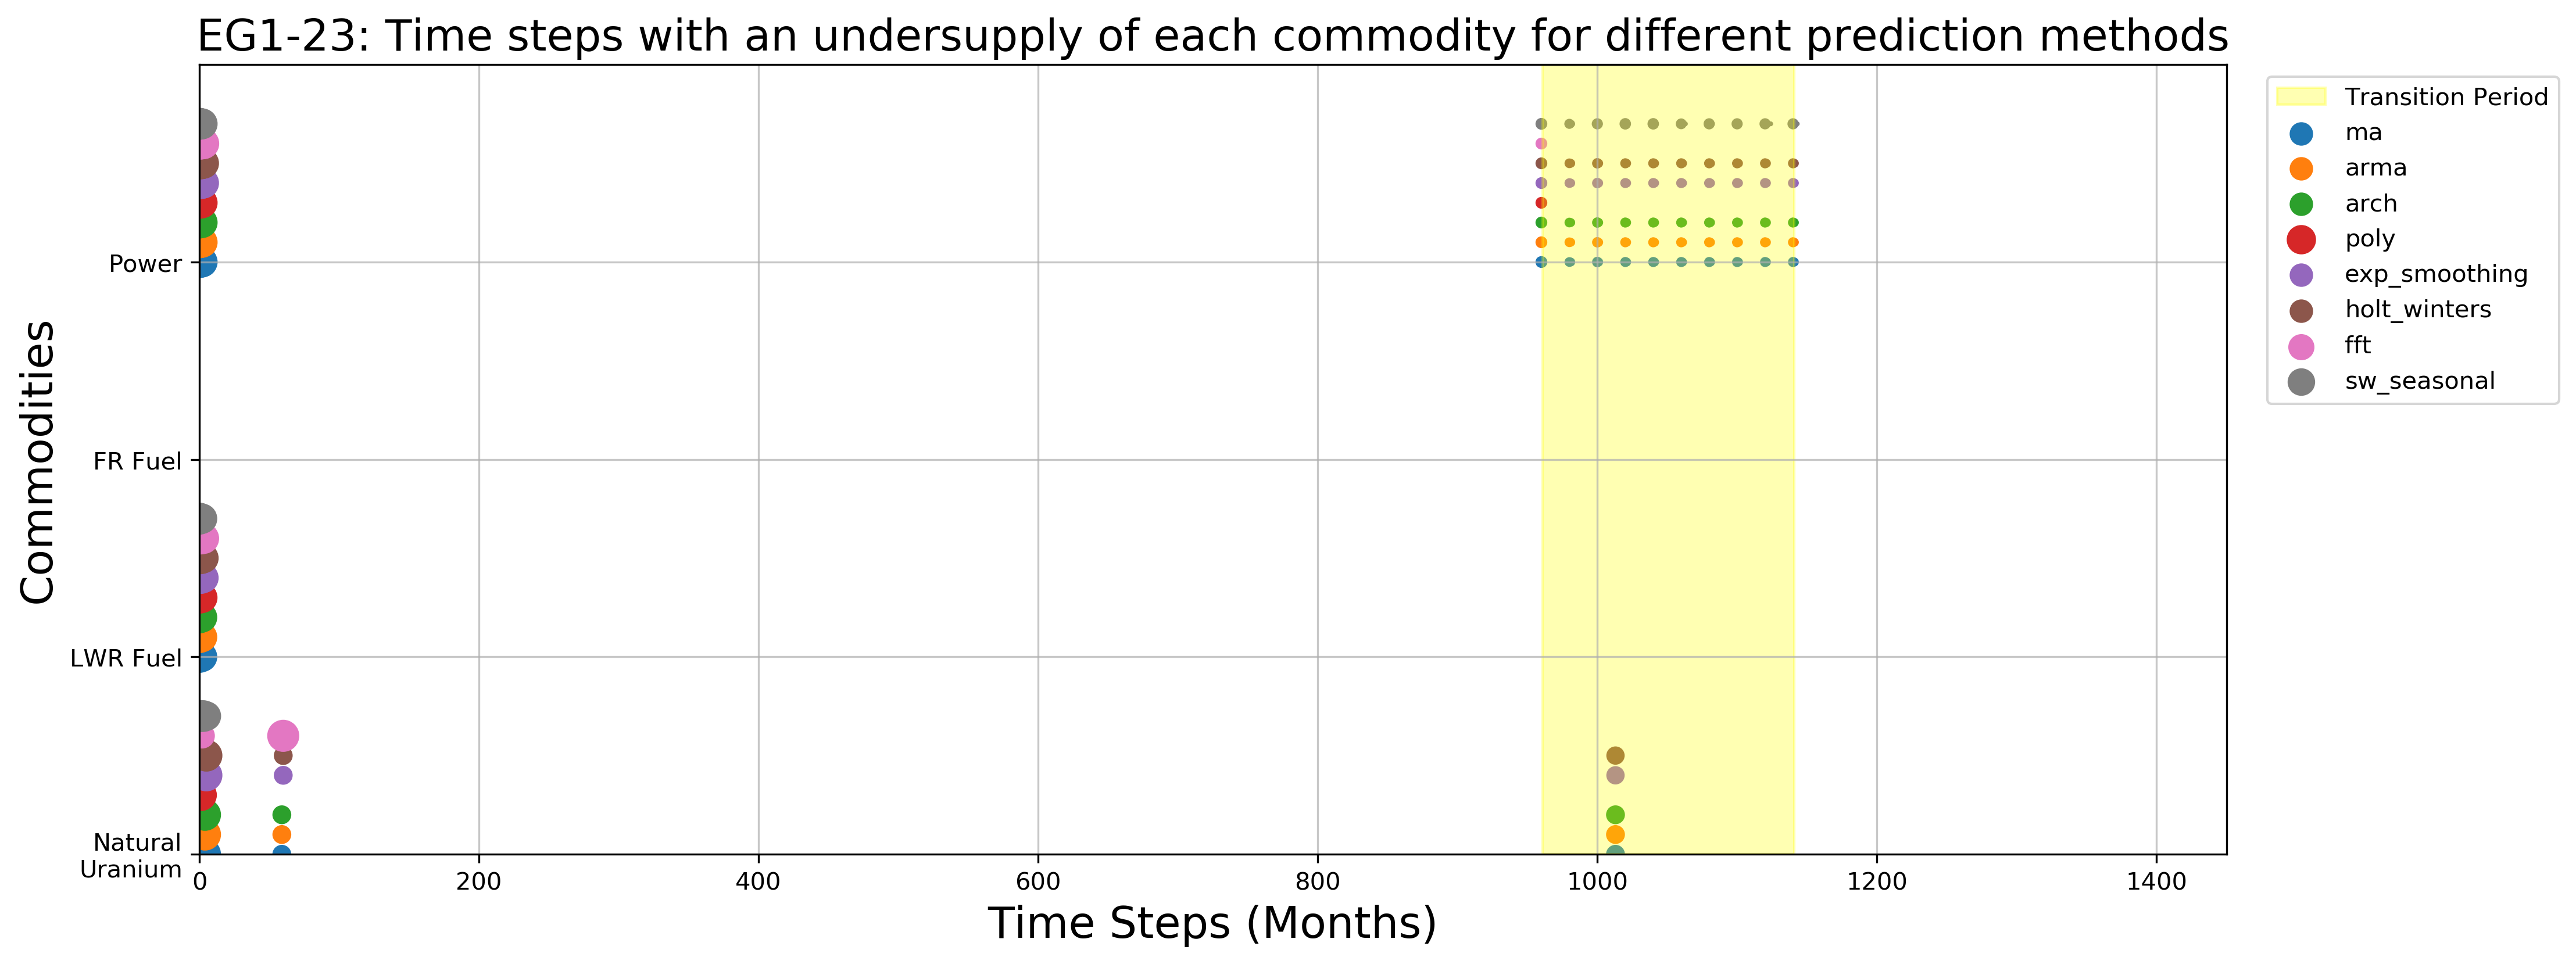
\includegraphics[width=\linewidth]{eg23-undersupply.png} 
		\caption{Time dependent undersupply of commodities in simulation }
		\label{fig:23undersupply}
	\end{subfigure}
	\vspace{1cm}
	\begin{subfigure}[t]{1.2\textwidth}
		\centering
		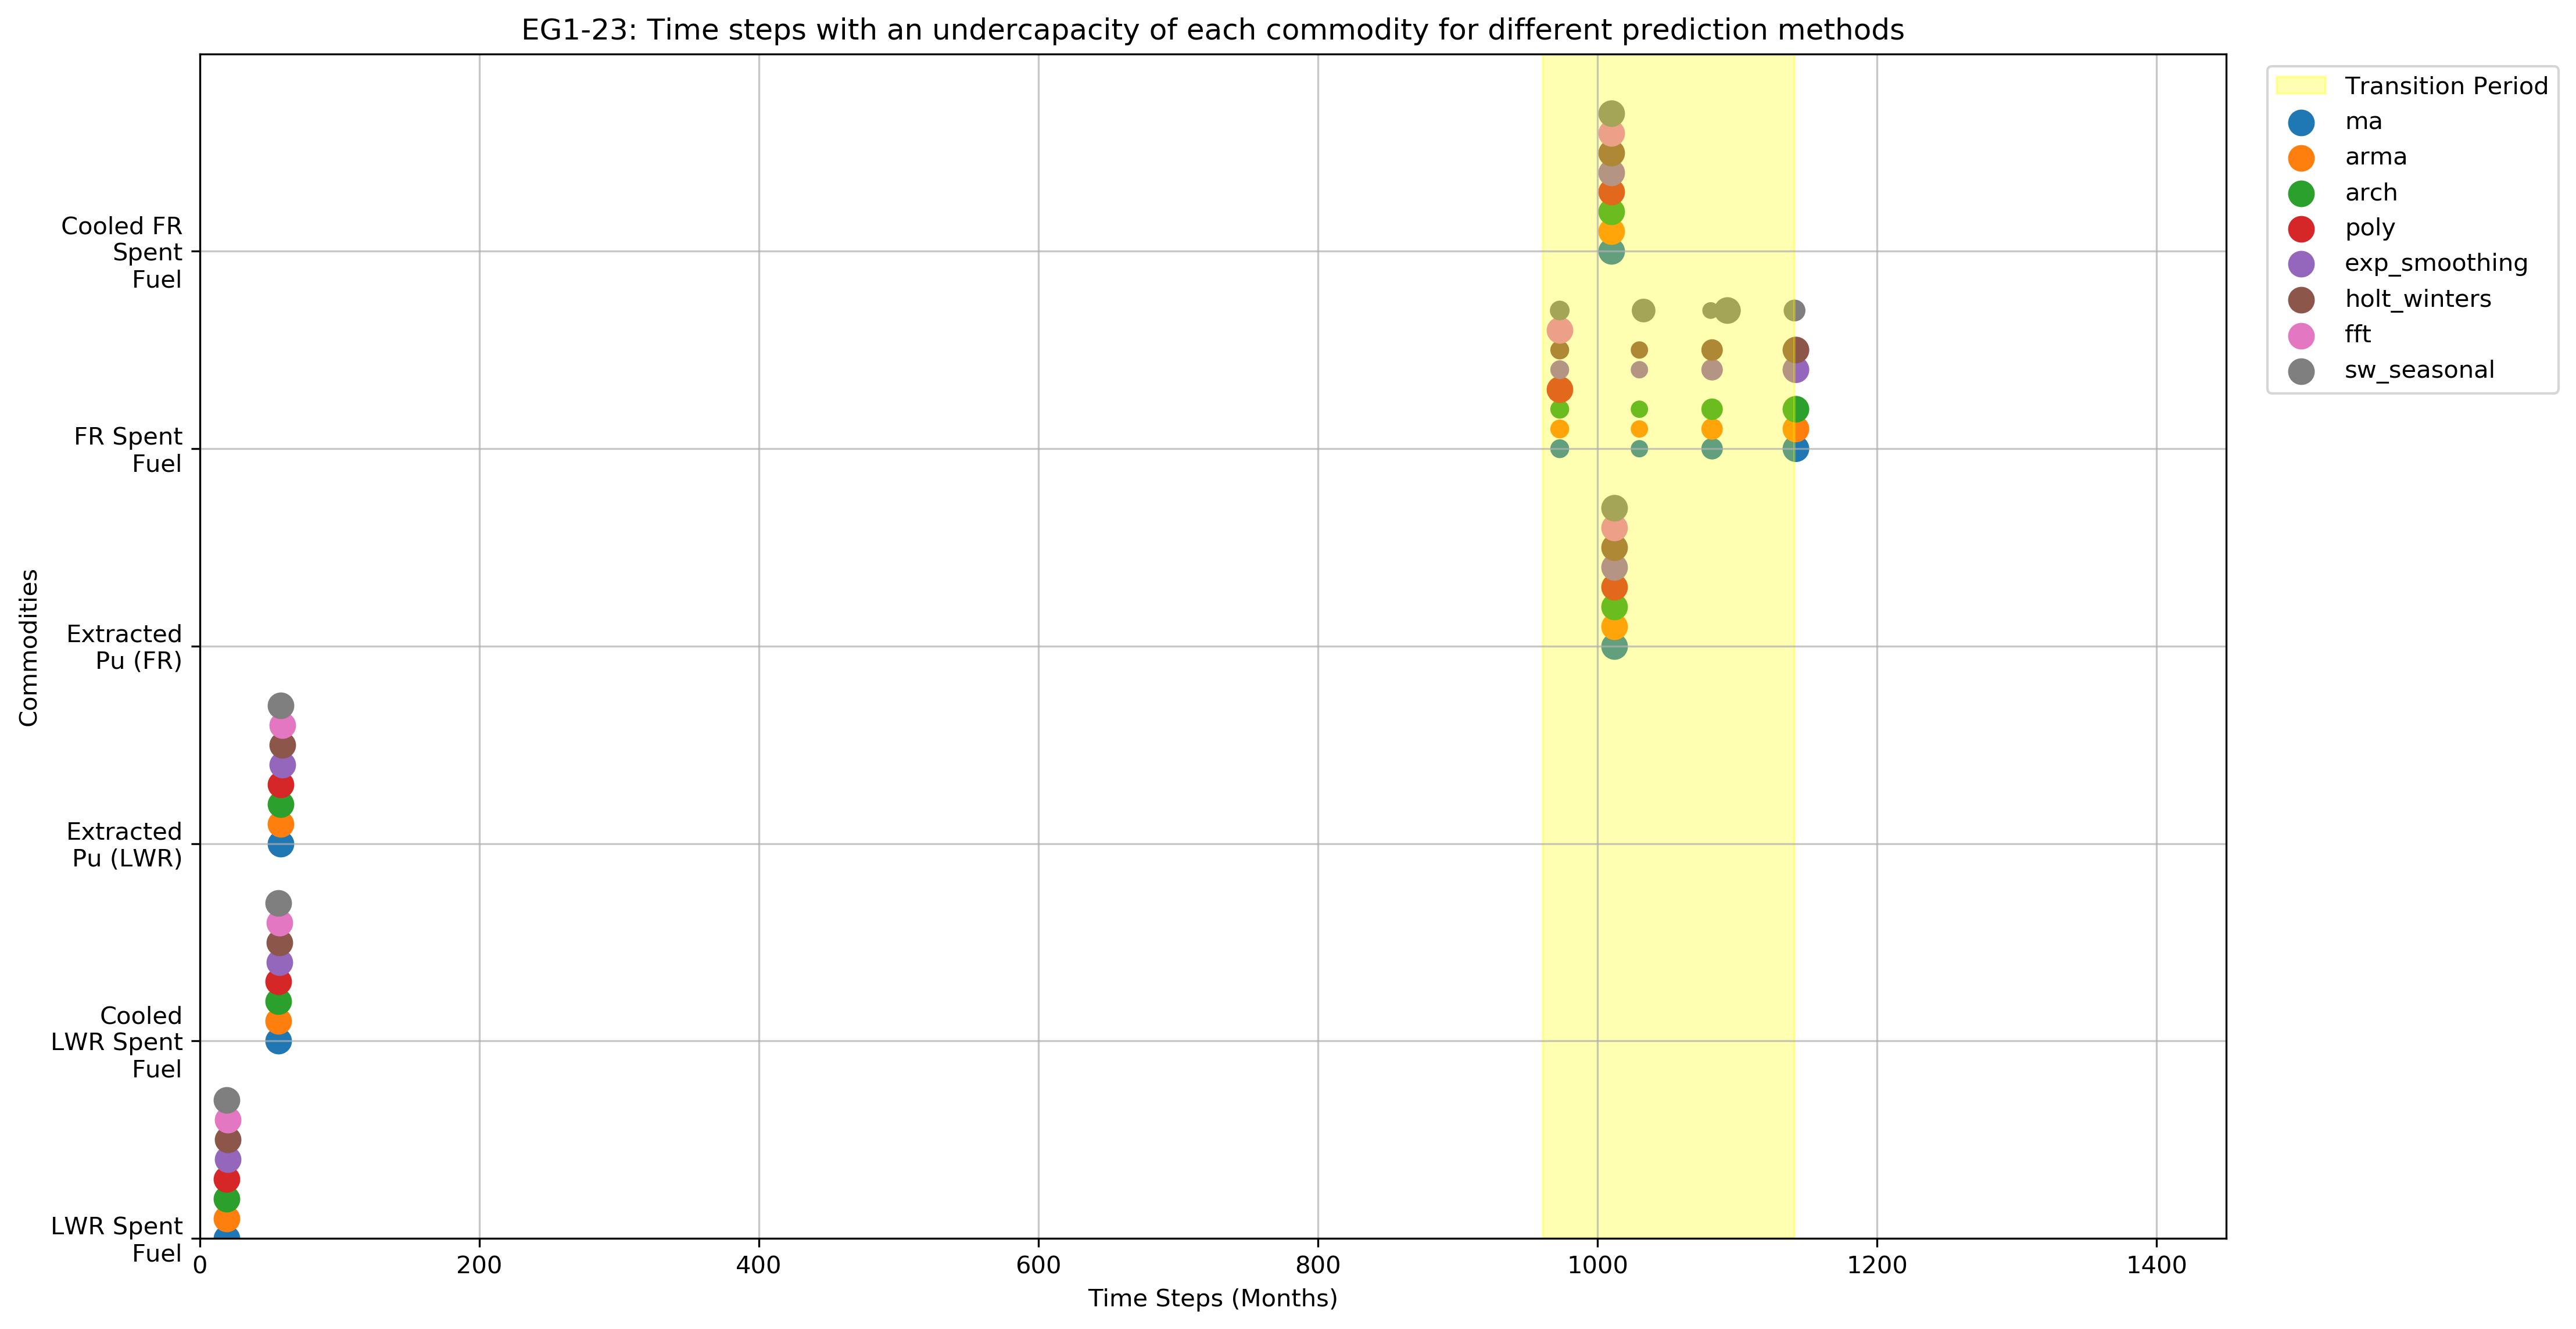
\includegraphics[width=\linewidth]{eg23-undercapacity.png} 
		\caption{Time dependent under-capacity of commodities in simulation }
		\label{fig:23undercapacity}
	\end{subfigure}
	\hfill
	\caption{
	EG01-23 transition scenario with constant power demand. 
	Each cross represents a time step in which there exists undersupply 
	or under-capacity of each commodity for varying prediction methods. 
	The size of each cross is proportional to the size of the undersupply.}
	\label{fig:eg23under}
\end{figure}

\begin{figure}[]
	\centering
	\begin{subfigure}[t]{1.2\textwidth}
		\centering
		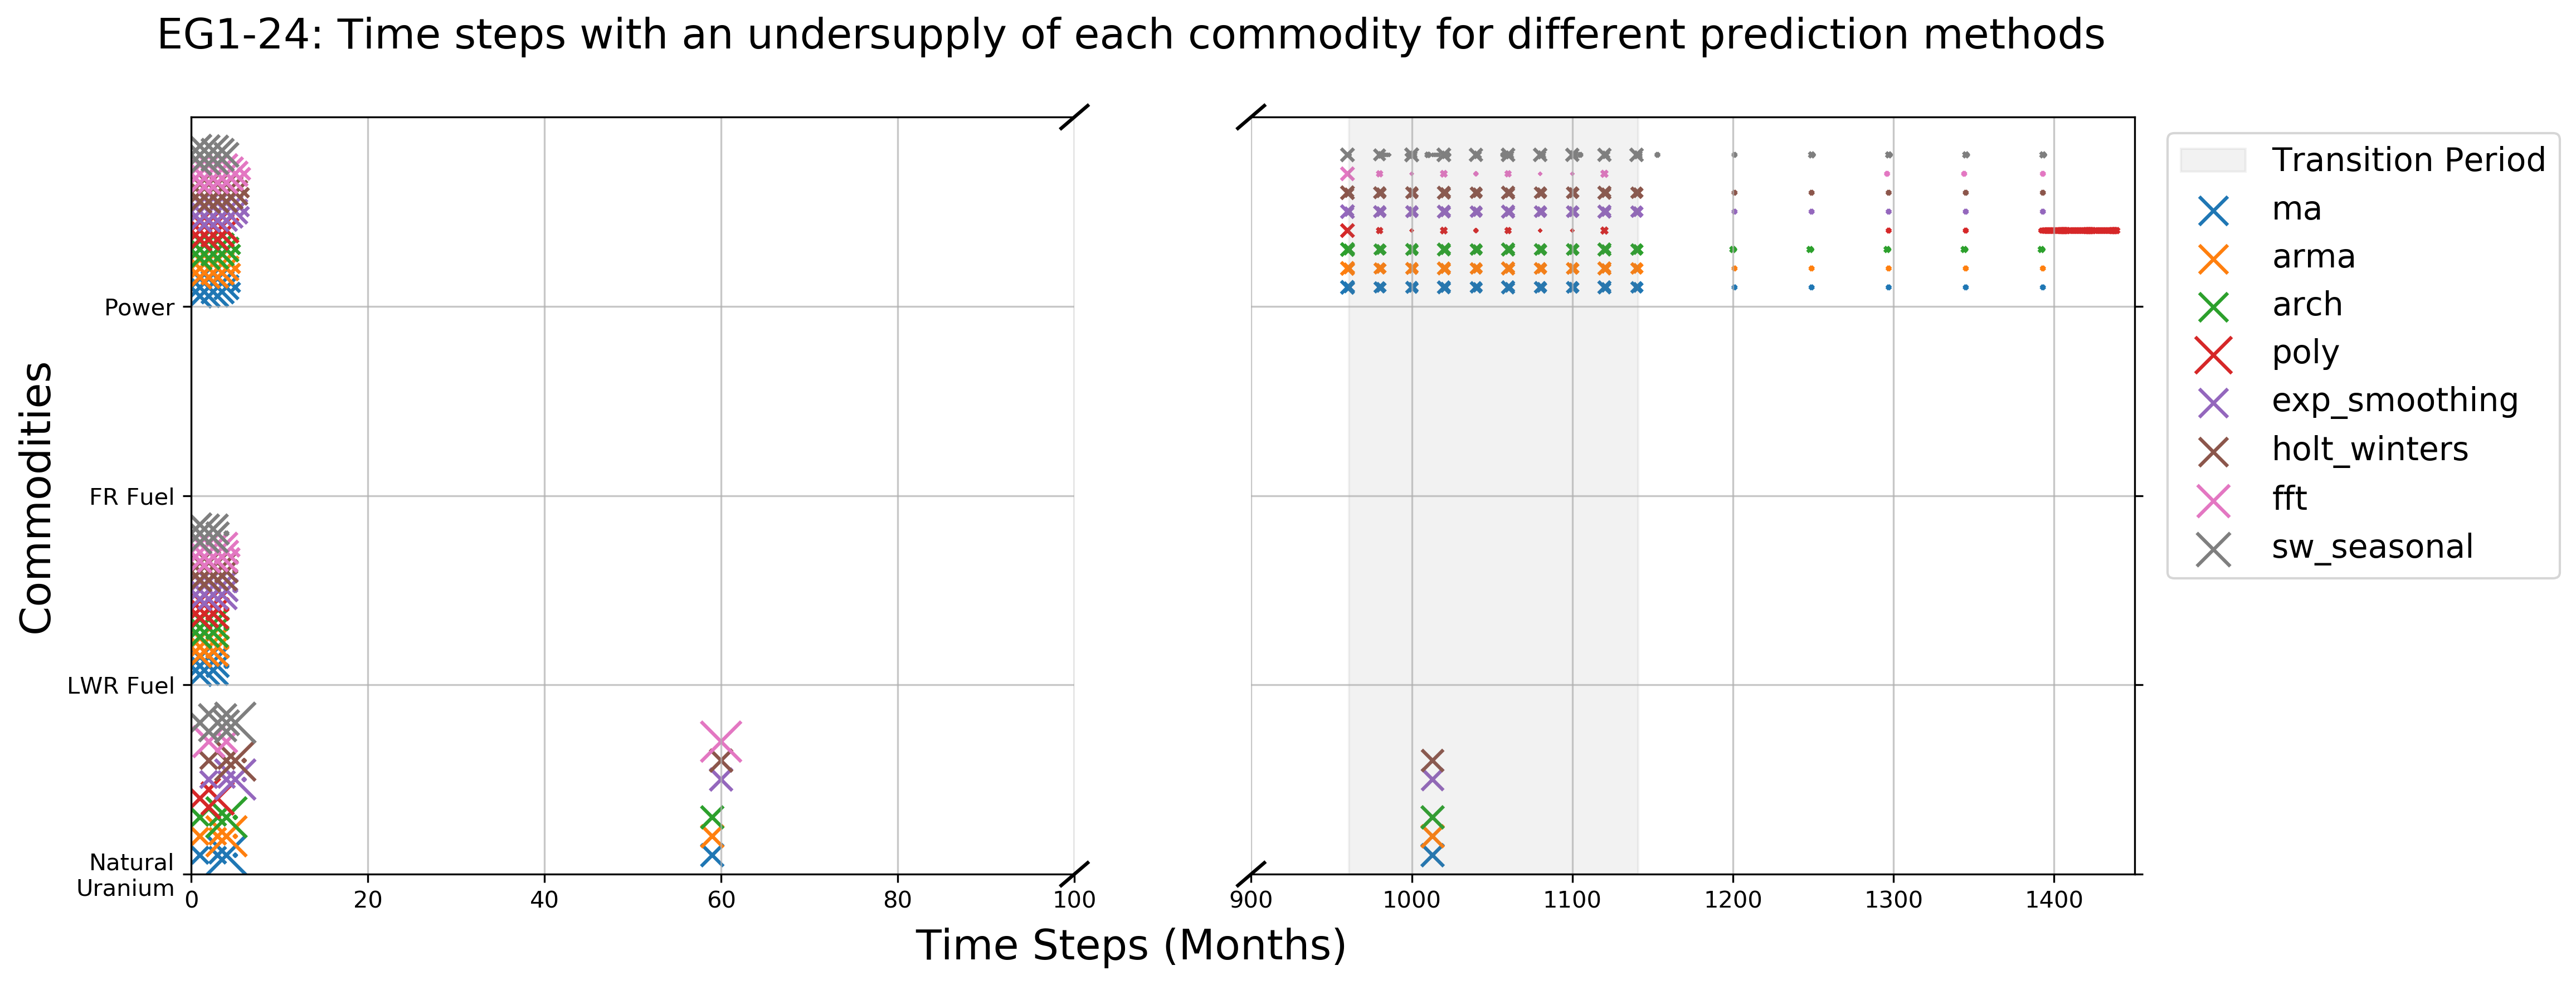
\includegraphics[width=\linewidth]{eg24-undersupply.png} 
		\caption{Time dependent undersupply of commodities in simulation }
		\label{fig:24undersupply}
	\end{subfigure}
	\vspace{1cm}
	\begin{subfigure}[t]{1.2\textwidth}
		\centering
		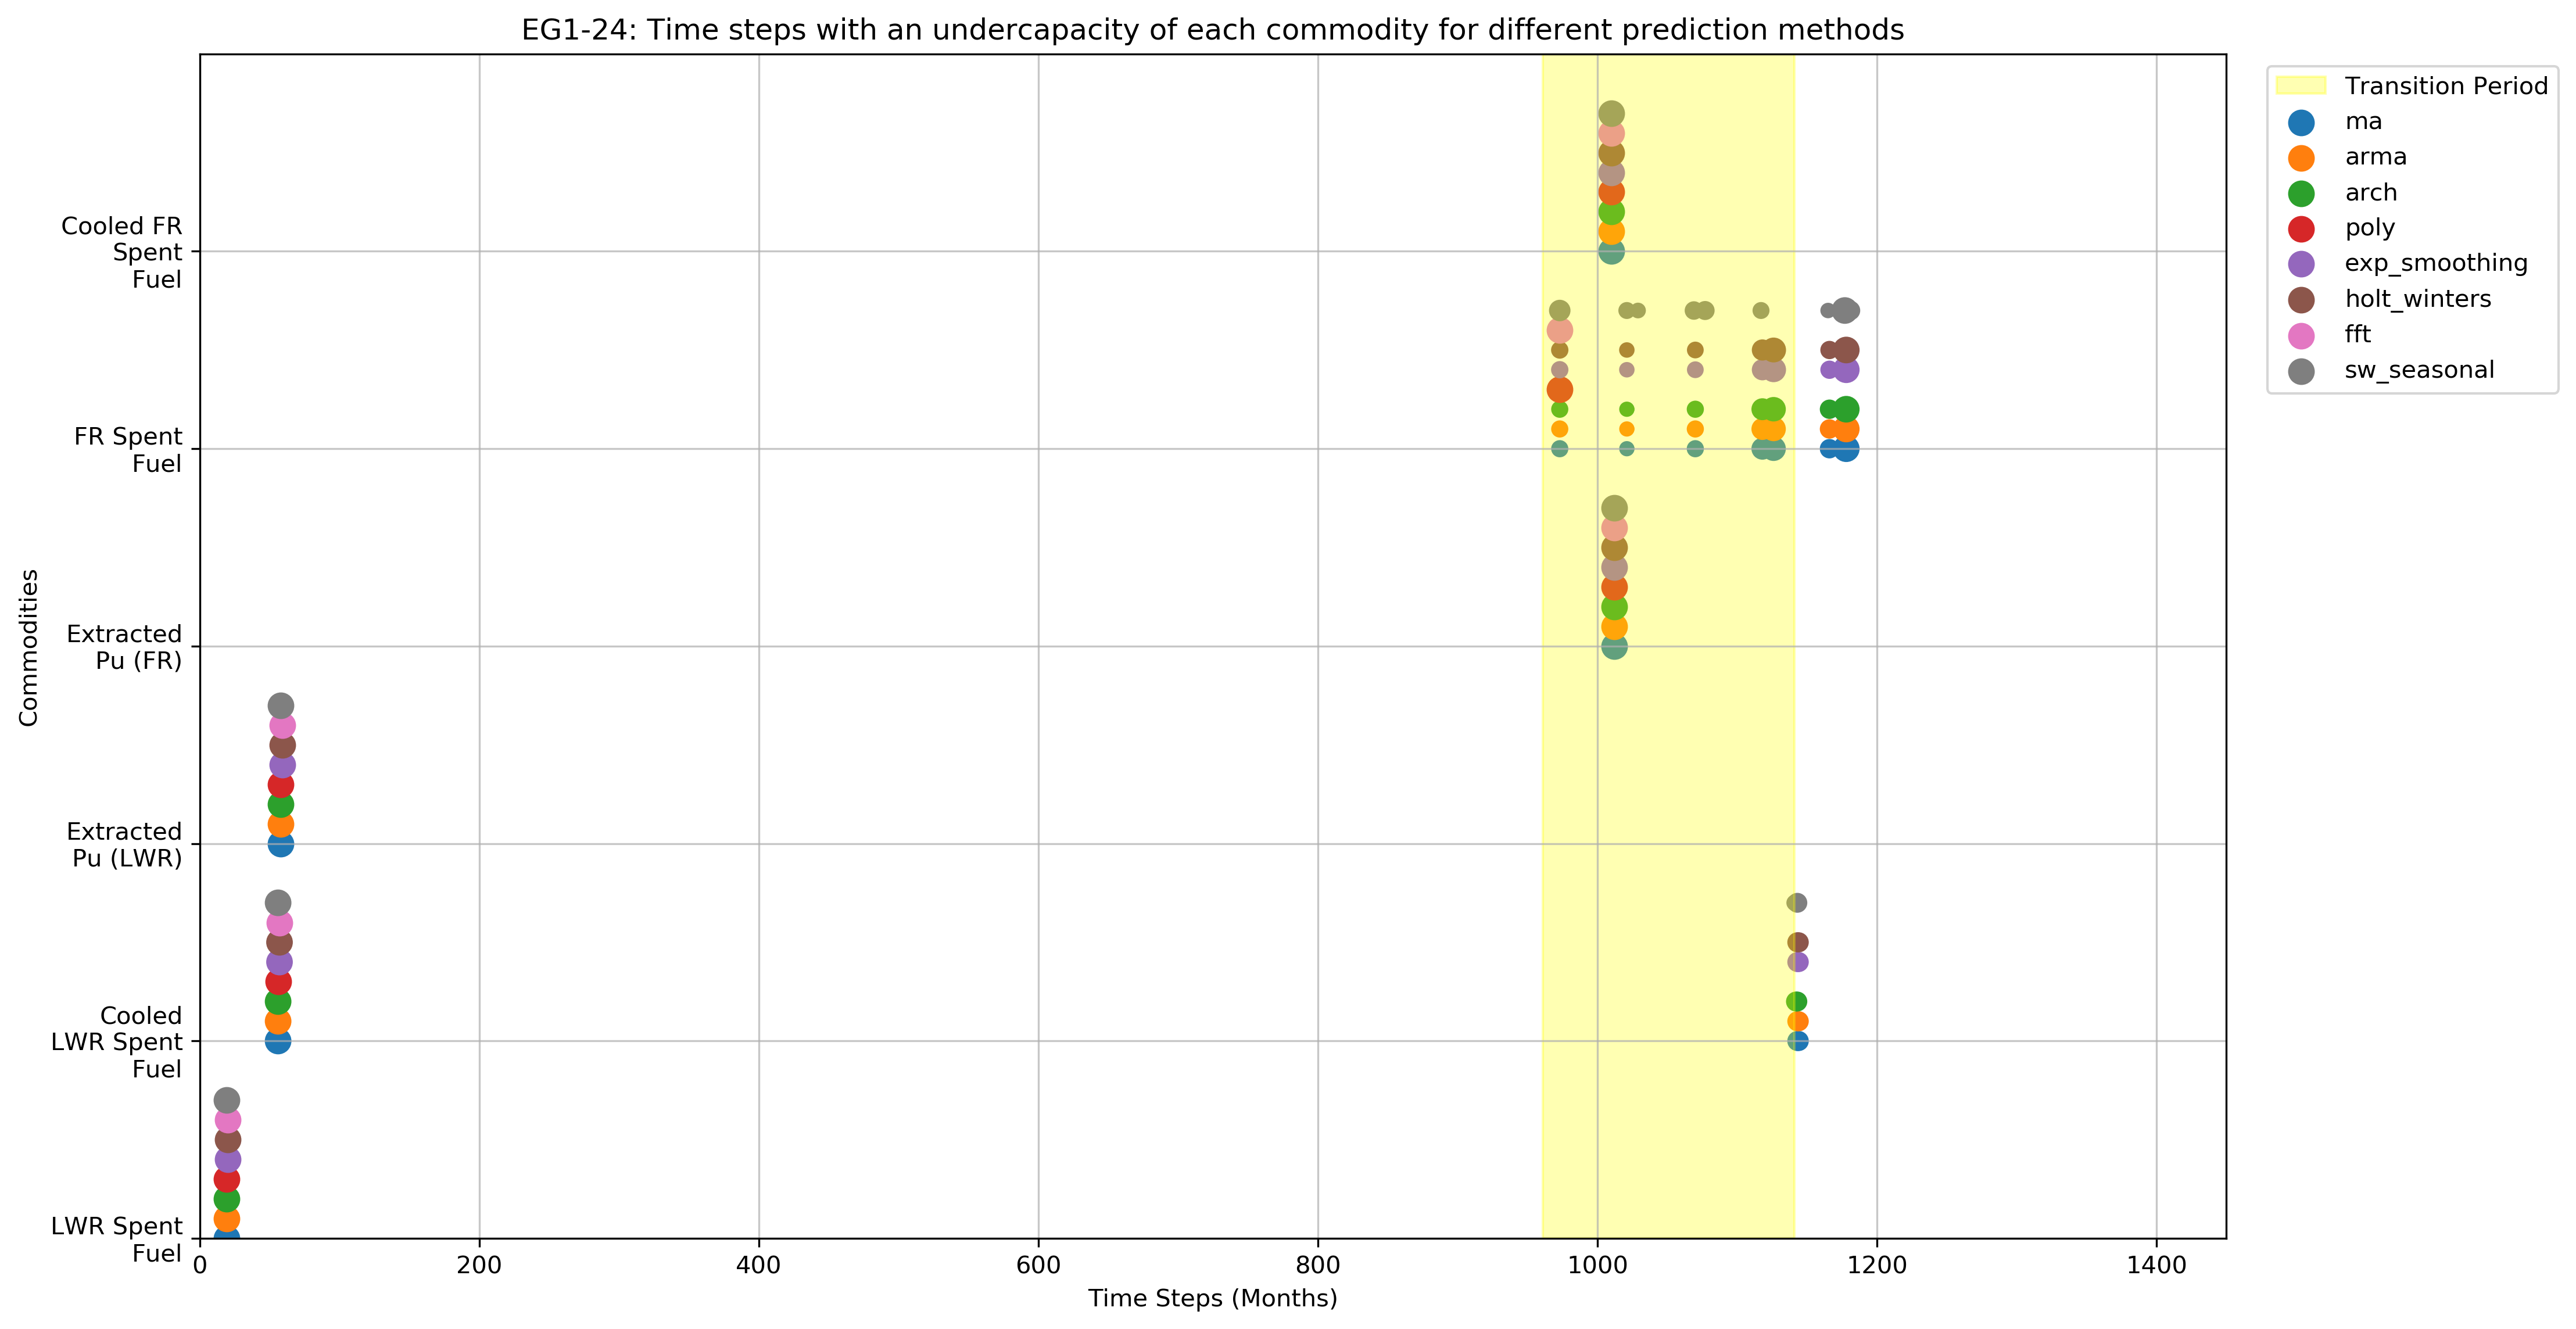
\includegraphics[width=\linewidth]{eg24-undercapacity.png} 
		\caption{Time dependent under-capacity of commodities in simulation }
		\label{fig:24undercapacity}
	\end{subfigure}
	\hfill
	\caption{
	EG01-24 transition scenario with linearly increasing power demand.
	Each cross represents a time step in which there exists undersupply 
	or under-capacity of each commodity for varying prediction methods. 
	The size of each cross is proportional to the size of the undersupply.}
	\label{fig:eg24under}
\end{figure}

\begin{table}[]
	\centering
		\caption{Undersupply and oversupply of power for EG01-EG23,24,29,30 
		transition scenarios for varying prediction methods.}
		\label{tab:all-power}
		\footnotesize
        \begin{tabularx}{\textwidth}{l|RRRR}
		\hline
		& \multicolumn{3}{|c}{\textbf{Power Undersupplied Time Steps}} \\ \hline
		\textbf{Algorithm} & \textbf{EG01-EG23 Constant Power}  & 
		\textbf{EG01-EG24 Linearly Increasing Power}   & \textbf{EG01-EG29 Constant Power} & 
		\textbf{EG01-EG30 Linearly Increasing Power} \\ \hline
		\texttt{MA}     		    & 26 	& 36  &  15  & 24 \\ 
		\texttt{ARMA}     	    & 26 	& 36  &  15  & 24\\ 
		\texttt{ARCH}     	    &  26 	& 36  &  15  & 21\\ 
		\texttt{POLY}      		&  6 	& 65  &  4 &  9\\ 
		\texttt{EXP-SMOOTHING} 	& 27 	& 37  & 16 & 25\\ 
		\texttt{HOLT-WINTERS}  	& 27 	& 37  & 16 & 25\\ 
		\texttt{FFT}       		& 8 	& 20  & 5 & 9\\ 
		\texttt{SW-SEASONAL}    & 36 	& 107 & 14 & 51\\ \hline
	\end{tabularx}
\end{table}

From Figures \ref{fig:eg23under}, \ref{fig:eg24under}, and Table 
\ref{tab:all-power}, we can see that the \texttt{POLY} method 
performs best for constant power transition scenarios, 
and the \texttt{FFT} method performs best for linearly increasing 
power transition scenarios. 
Undersupply and under-capacity of commodities occur during two main time periods: 
initial demand for the commodity and during the transition period.
To further \deploy's primary objective of minimizing the power undersupply, 
sensitivity analysis of the power supply buffer is conducted 
with the best-performing prediction method for each transition scenario.  

\subsection{Sensitivity Analysis}
We conducted a sensitivity analysis of the power buffer size for the
EG01-EG23, EG01-24, EG01-29, and EG01-30 transition scenarios. 
Varying the power buffer size does not impact the number of 
undersupply time steps for the EG01-EG23 and EG01-EG29 constant 
power demand transition scenarios with the \texttt{POLY} prediction method.
In Table \ref{tab:all-power}, there are 6 and 4 time steps
in which there is power undersupply for the EG01-EG23 and EG01-29 
transition scenarios, respectively. 
As seen in figure \ref{fig:eg23under}, these undersupply time 
steps occur at the beginning of the simulation and for one 
time step when the transition begins. 
We expected this since without time-series data 
at the beginning of the simulation, \deploy takes a few 
time steps to collect time-series data about power demand 
to predict and start deploying reactor and supporting 
fuel cycle facilities. 
When the transition begins, power is undersupplied for one 
time step, following this, \deploy accounts for the 
undersupply by deploying facilities to meet power demand.
Therefore, we minimized the power undersupply for constant 
power EG01-EG23 and EG01-EG29 transition scenarios with 
a 0MW power supply buffer. 

We varied the power buffer size for the EG01-24 and EG01-30 
linearly increasing power demand transition scenarios. 
Figures \ref{fig:eg24-bufplot}, \ref{fig:eg30-bufplot}, 
and Table \ref{tab:buff_size} 
show that increasing the buffer size decreases the number of 
power undersupply time steps. 
For EG01-24, the cumulative undersupply plateaus at 6000MW, 
and for EG01-30, the cumulative undersupply is smallest 
for a buffer size of 8000MW.
As seen from Figures \ref{fig:eg24-dotplot} and 
\ref{fig:eg30-dotplot}, these undersupply time 
steps occur at the beginning of the simulation and for one 
time step when the transition begins. 
We expected this since without time-series data 
at the beginning of the simulation, \deploy takes a few 
time steps to collect time-series data about power demand 
to predict and start deploying reactor and supporting 
fuel cycle facilities. 
Therefore, a buffer of 6000MW and 8000MW minimizes 
the power undersupply for EG01-EG24 and EG01-EG30, respectively.

\begin{figure}[]
	\centering
	\begin{subfigure}[t]{0.8\textwidth}
		\centering
		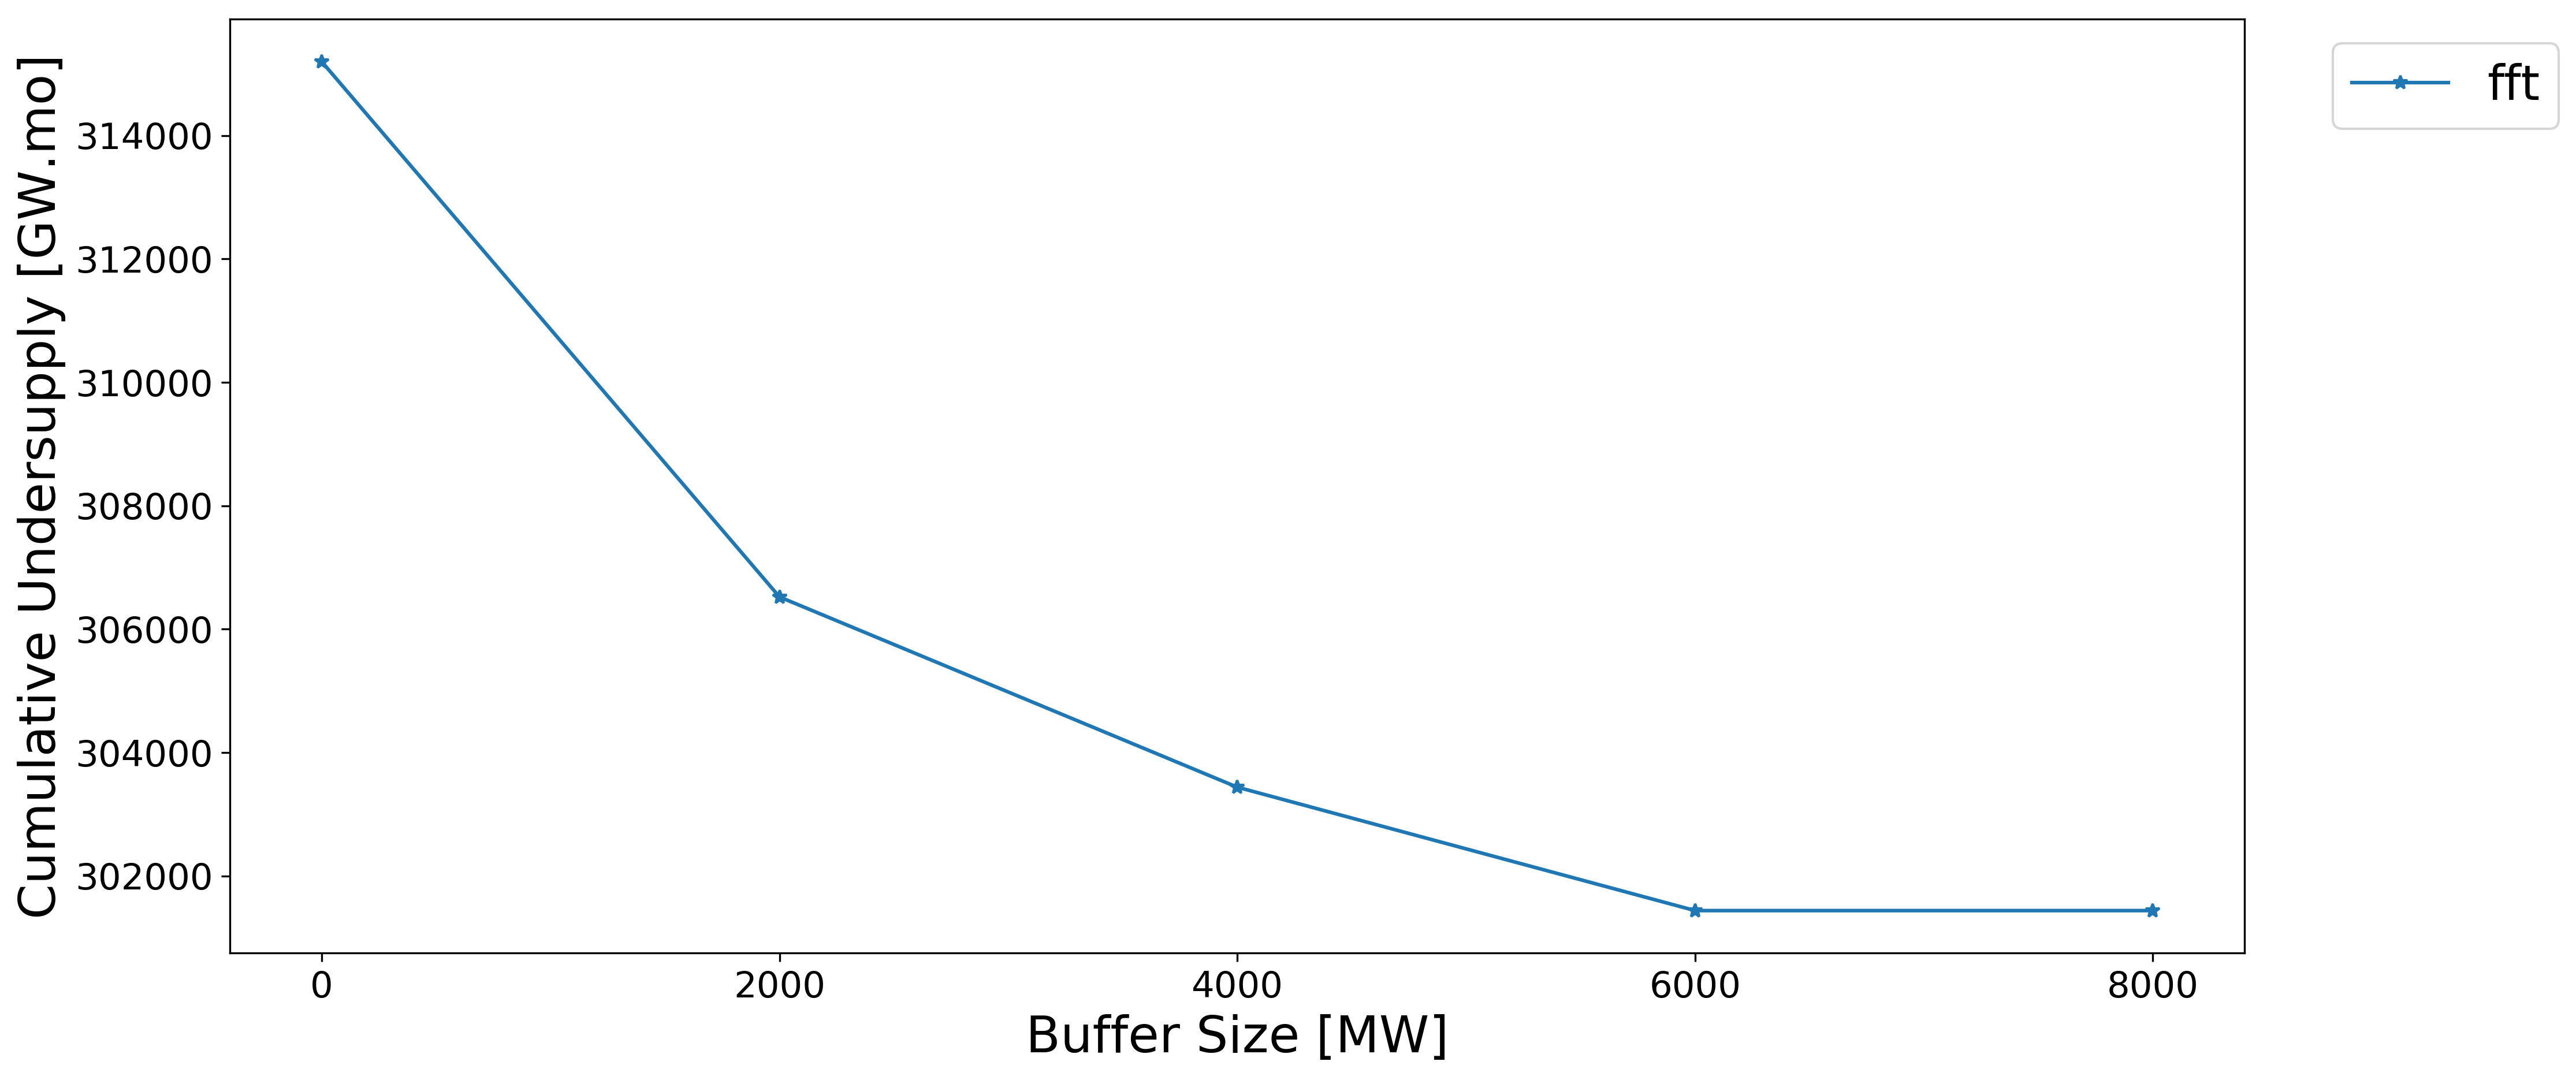
\includegraphics[width=\linewidth]{24-sens-buffer.png} 
		\caption{EG01-24: Power buffer size vs. cumulative undersupply}
		\label{fig:eg24-bufplot}
	\end{subfigure}
	\vspace{1cm}
	\begin{subfigure}[t]{0.8\textwidth}
		\centering
		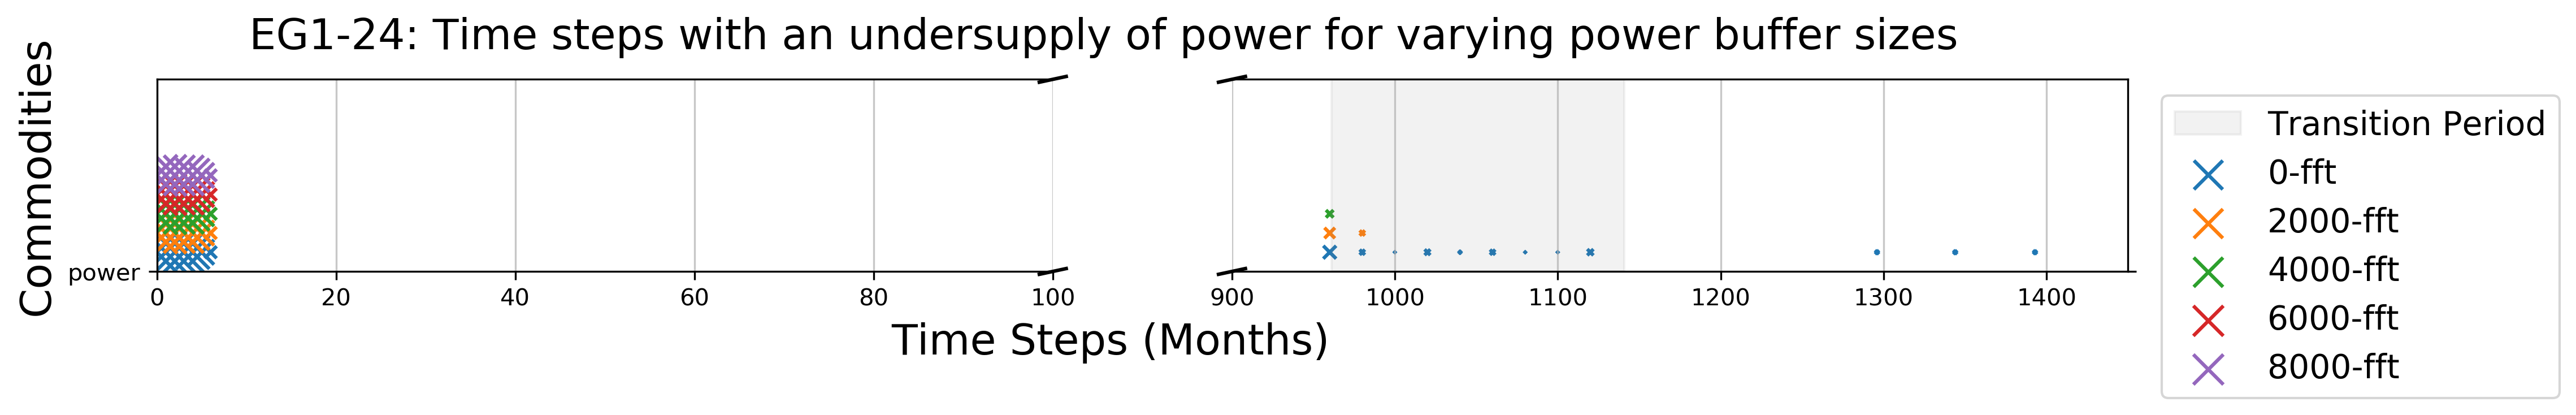
\includegraphics[width=\linewidth]{eg24-sa.png} 
		\caption{EG01-24: Time-dependent undersupply of power for varying power buffer sizes}
		\label{fig:eg24-dotplot}
	\end{subfigure}
	\begin{subfigure}[t]{0.8\textwidth}
		\centering
		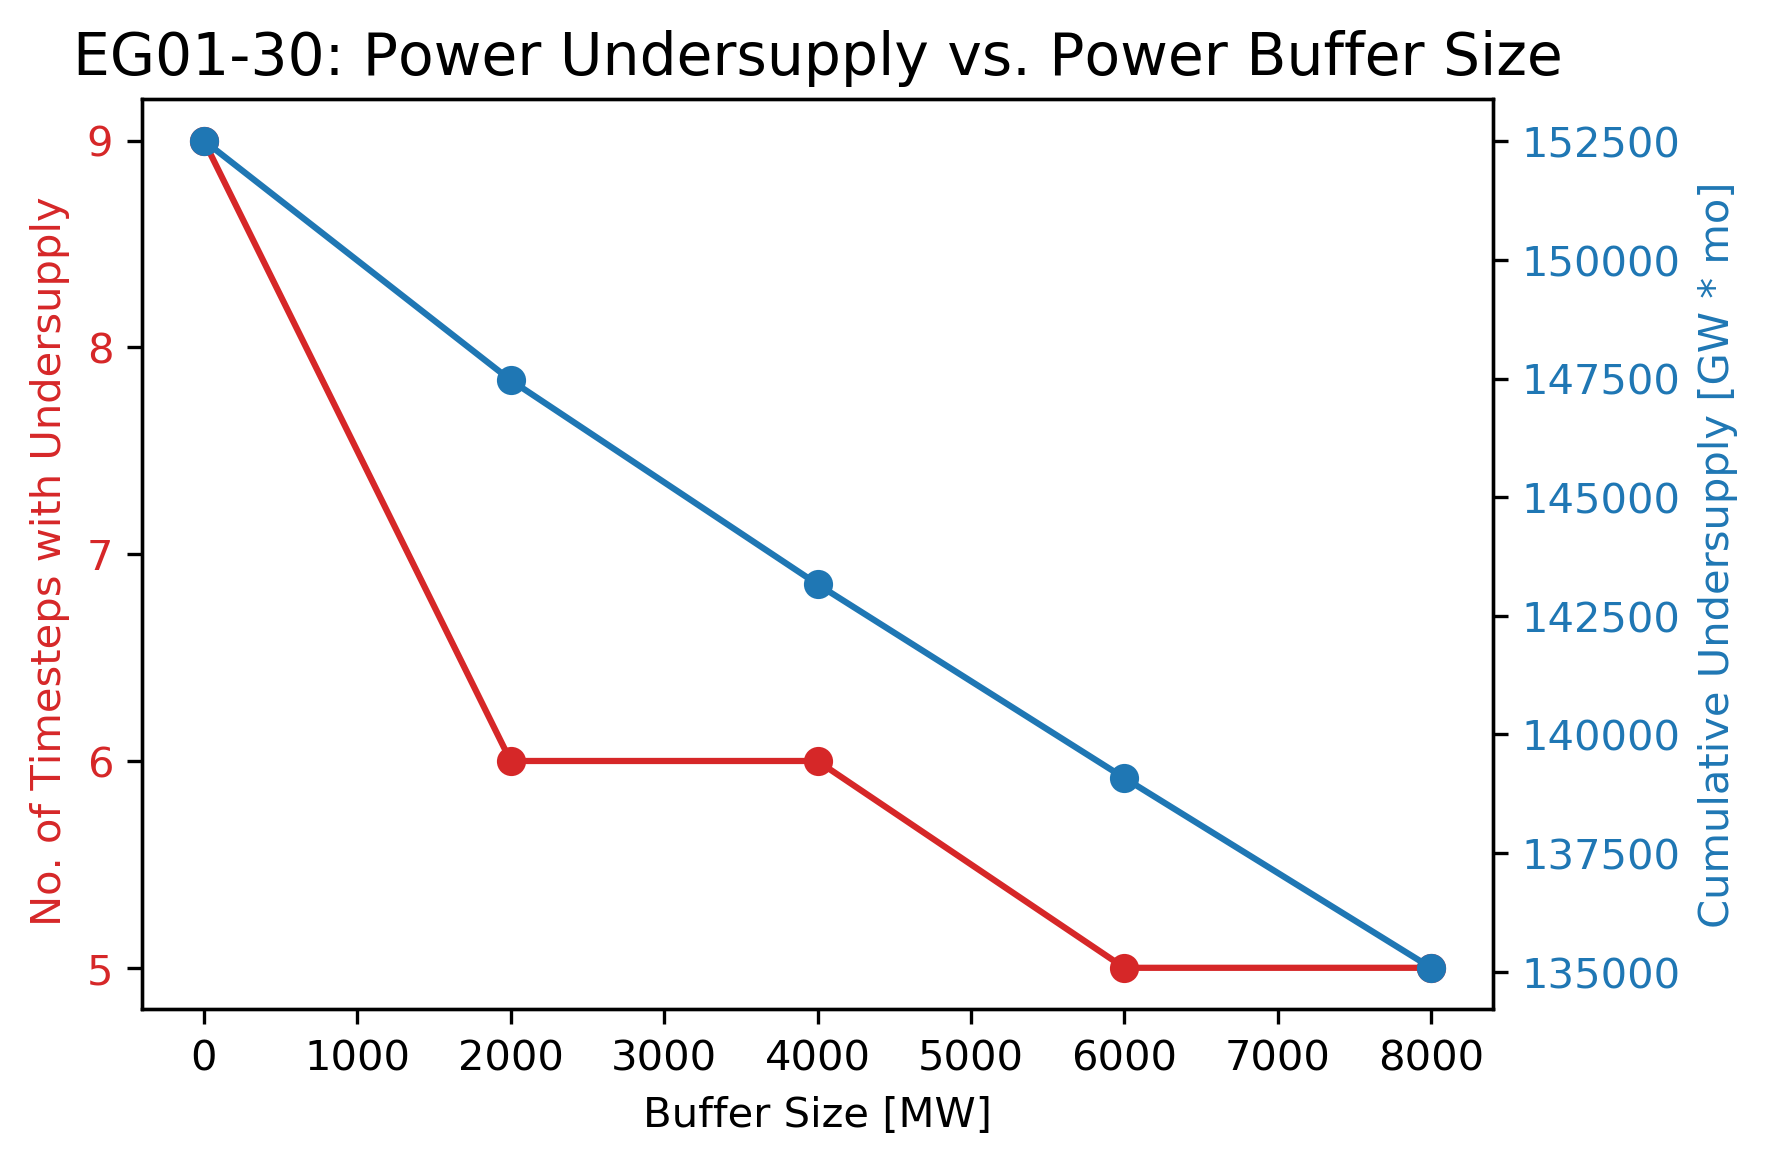
\includegraphics[width=\linewidth]{30-sens-buffer.png} 
		\caption{EG01-30: Power buffer size vs. cumulative undersupply}
		\label{fig:eg30-bufplot}
	\end{subfigure}
	\begin{subfigure}[t]{0.8\textwidth}
		\centering
		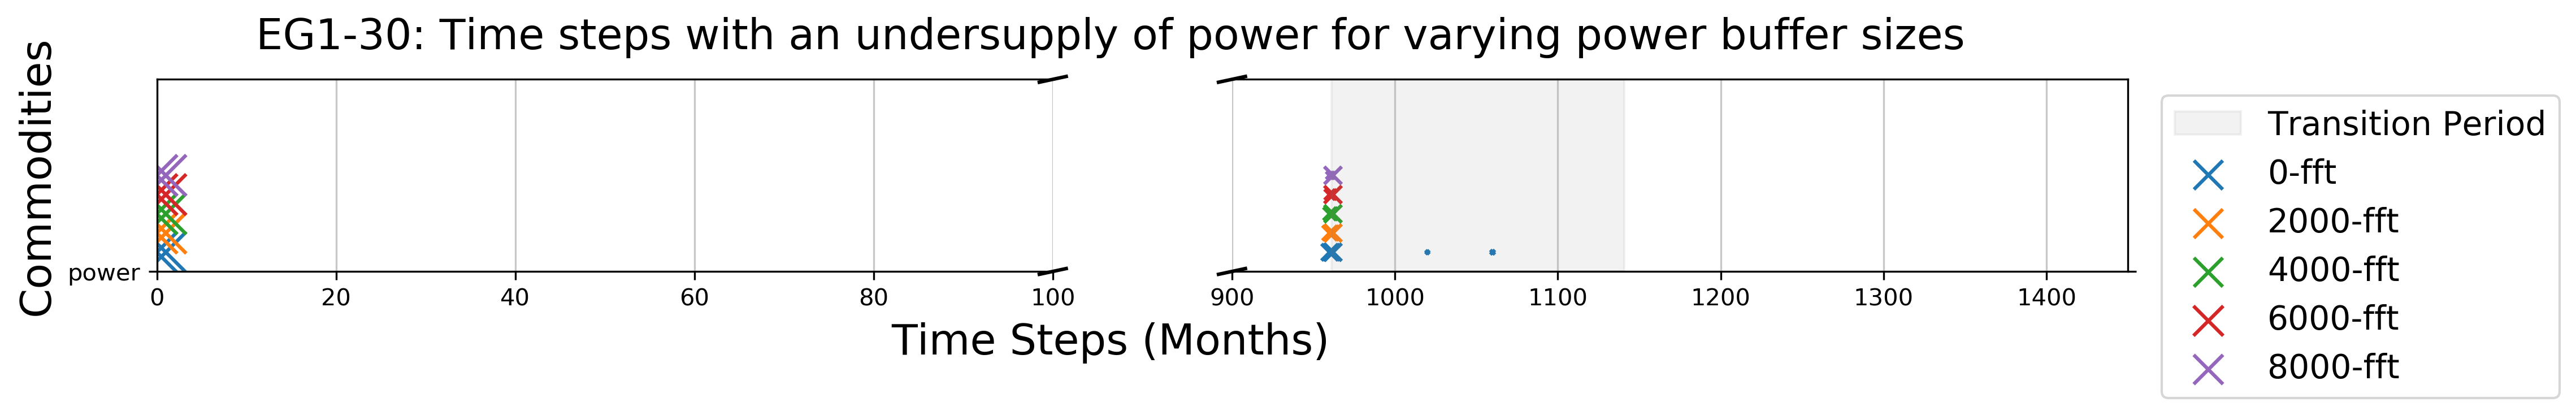
\includegraphics[width=\linewidth]{eg30-sa.png} 
		\caption{EG01-30: Time-dependent undersupply of power for varying power buffer sizes}
		\label{fig:eg30-dotplot}
	\end{subfigure}
	\hfill
	\caption{The effect of sensitivity analysis of power buffer size on cumulative 
	undersupply of power for EG01-EG24 and EG01-EG30 transition scenarios 
	with linearly increasing power demand using the \texttt{FFT} prediction method.}
	\label{fig:sabuffer}
\end{figure}

\begin{table}[h]
	\centering
	\caption{The effect of sensitivity analysis of power buffer size on cumulative 
	undersupply of power for EG01-EG24 and EG01-EG30 transition scenarios with linearly 
	increasing power demand using the \texttt{FFT} prediction method.}
	\label{tab:buff_size}
	\footnotesize
		\begin{tabular}{l|lrr}
                \hline
        \textbf{Buffer [MW]}     & \textbf{Undersupply}             & \textbf{EG01-24}   & \textbf{EG01-30} \\
		\hline
		\textbf{0}             & Time steps $[\#]$ & 20 & 9\\  
                      & Energy $[GW\cdot mo]$    & 315791 & 152517 \\ \hline
		\textbf{2000}          & Undersupplied $[\#]$ & 9 & 6 \\  
        	      & Energy $[GW\cdot mo]$    & 306520 & 147166 \\ \hline
        \textbf{4000}          & Time steps $[\#]$ & 8 & 6 \\  
				  & Energy $[GW\cdot mo]$    & 303438 & 143166 \\ \hline
		\textbf{6000}          & Time steps $[\#]$ & 7 & 5 \\  
		& Cumulative $[GW]$    & 303438 & 139083 \\ \hline
        \textbf{8000}          & Time steps $[\#]$ & 7 & 5  \\  
	              & Energy $[GW\cdot mo]$    & 303438 & 135083 \\ \hline
	\end{tabular}
\end{table}

\subsection{Best Performance Models}
Table \ref{tab:bestinputs} shows the \deploy input parameters for
EG01-EG23, EG01-EG24, EG01-EG29, and EG01-EG30 transition scenarios
that minimize the undersupply of power and 
undersupply and under-capacity of the other commodities
in the simulation. 
The need for commodity supply buffers is a reflection of reality
in which a supply buffer is usually maintained to ensure 
continuity in the event of an unexpected failure in the supply chain.

Figures \ref{fig:23stack} and \ref{fig:30stack} show
time-dependent deployment of reactor and supporting facilities for 
the EG01-23 constant power demand and EG01-30 linearly increasing power demand 
transition scenarios, respectively. 
\deploy automatically deploys reactor and supporting facilities 
to set up a supply chain to meet power demand
during a transition from \glspl{LWR} to \glspl{SFR} for EG01-23, 
and from \glspl{LWR} to \gls{MOX} \glspl{LWR} and \glspl{SFR} for 
EG01-30. 
EG01-24 and EG01-29 facility deployment plots are similar to 
EG01-23 and EG01-30, respectively, therefore they are not shown. 

\begin{table}[]
	\resizebox{\textwidth}{!}{%
	\begin{tabular}{l|l|c|l|l|l}
	\hline
	\multirow{2}{*}{}                         & \multicolumn{1}{c|}{\multirow{2}{*}{\textbf{Input Parameter}}} & \multicolumn{4}{c}{\textbf{Simulation Description}}                                                                                                                                                                                                                                                       \\ \cline{3-6} 
											  & \multicolumn{1}{c|}{}                                          & \multicolumn{1}{l|}{\textbf{EG01-23}}                                                                 & \textbf{EG01-24}                  & \textbf{EG01-29}                 &\textbf{EG01-30}                                                  \\ \hline
	\multirow{4}{*}{\textbf{Required}} & Demand driving commodity                                       & \multicolumn{4}{c}{Power}                                                                                                                                                                                                                                                                                 \\ \cline{2-6} 
											  & Demand equation [MW]                                               & \multicolumn{1}{l|}{60000}                                                                                & $60000 + 250t/12$ & 60000                     &     $60000 + 250t/12$                                       \\ \cline{2-6} 
											  & Prediction method                                              & \texttt{POLY}       & \texttt{FFT}             & \texttt{POLY}         &  \texttt{FFT}    \\ \cline{2-6} 
											  & Deployment Driving Method                                      & \multicolumn{4}{c}{Installed Capacity}                                                                                                                                                                                                                                                                    \\ \hline
	\multirow{2}{*}{\textbf{Optional}} & Buffer type                                                    & \multicolumn{4}{c}{Absolute}                                                                                                                                                                                                                                                               \\ \cline{2-6} 
											  & Power Buffer size [MW]                                                   & 0 & 6000 & 0 & 8000 \\ \hline
	\end{tabular}%
	}
	\caption{\deploy's input parameters for EG01-EG23, EG01-EG24, EG01-EG29, and 
	EG01-EG30 transition scenarios
	that minimizes undersupply of power and minimizes 
	the undersupply and under-capacity of the other facilities. }
	\label{tab:bestinputs}
	\end{table}

\begin{figure}[]
	\centering
	\begin{subfigure}[t]{1.2\textwidth}
		\centering
		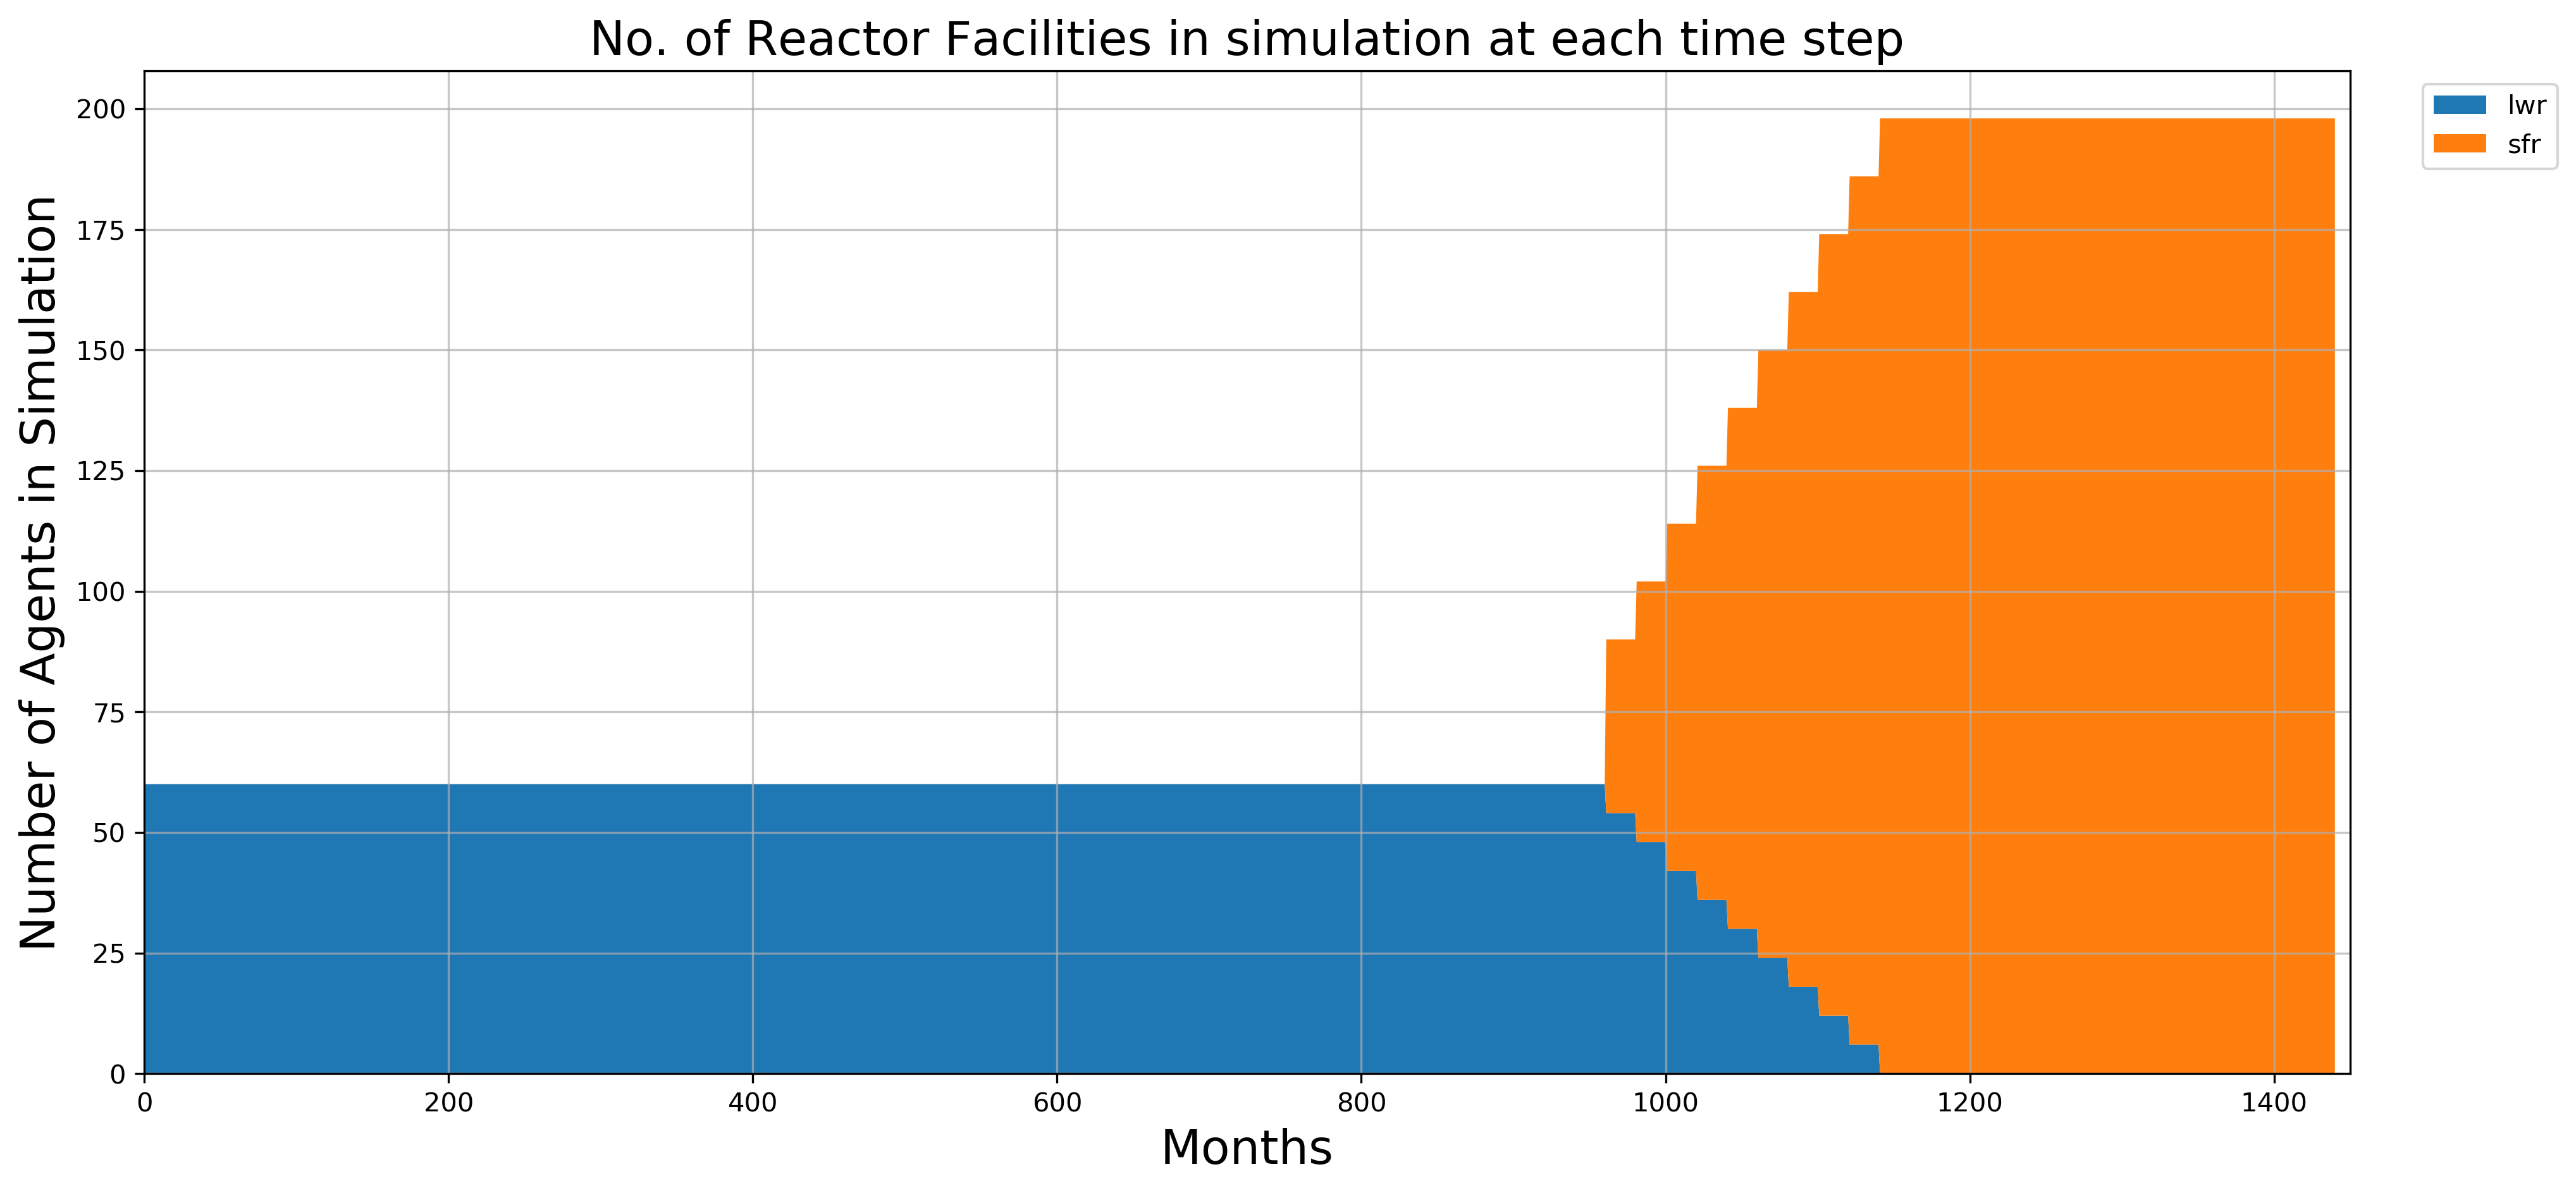
\includegraphics[width=\linewidth]{eg23-stack_reactor.png} 
		\caption{EG01-23: Reactor Deployment}
		\label{fig:23reactor}
	\end{subfigure}
	\vspace{1cm}
	\begin{subfigure}[t]{1.2\textwidth}
		\centering
		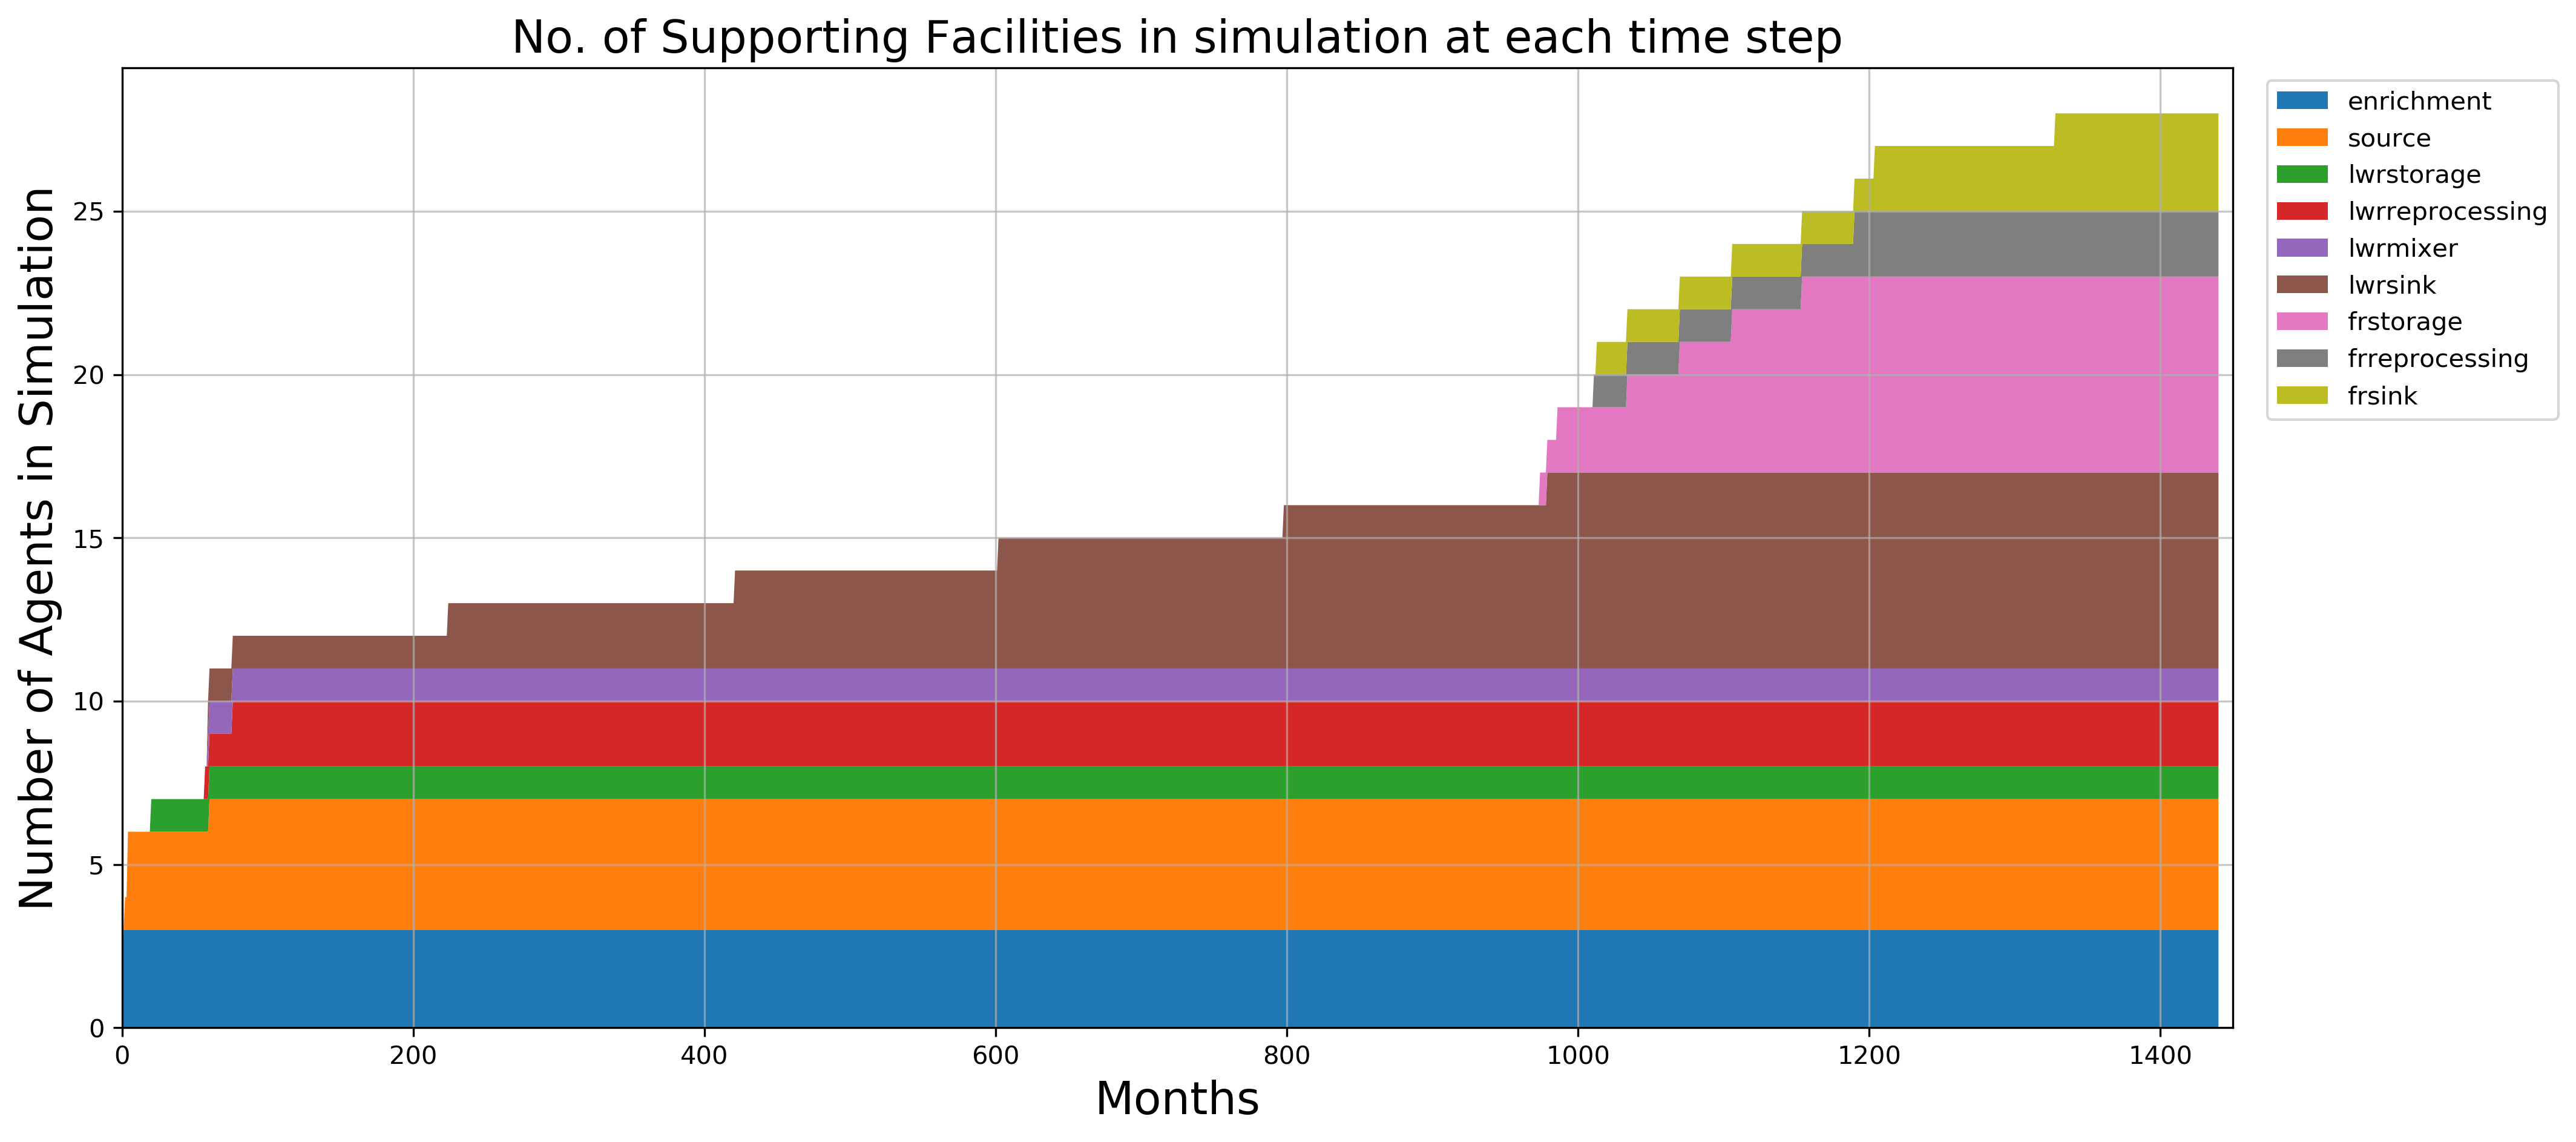
\includegraphics[width=\linewidth]{eg23-stack_support.png} 
		\caption{EG01-23: Supporting Facility Deployment}
		\label{fig:23support}
	\end{subfigure}
	\hfill
	\caption{Time dependent deployment of reactor and supporting facilities in 
	the EG01-23 constant power demand transition scenario. 
	\deploy automatically deploys reactor and supporting facilities 
	to setup a supply chain to meet constant power demand of $60000$ MW
	during a transition from \glspl{LWR} to \glspl{SFR}. }
	\label{fig:23stack}
\end{figure}

\begin{figure}[]
	\centering
	\begin{subfigure}[t]{1.2\textwidth}
		\centering
		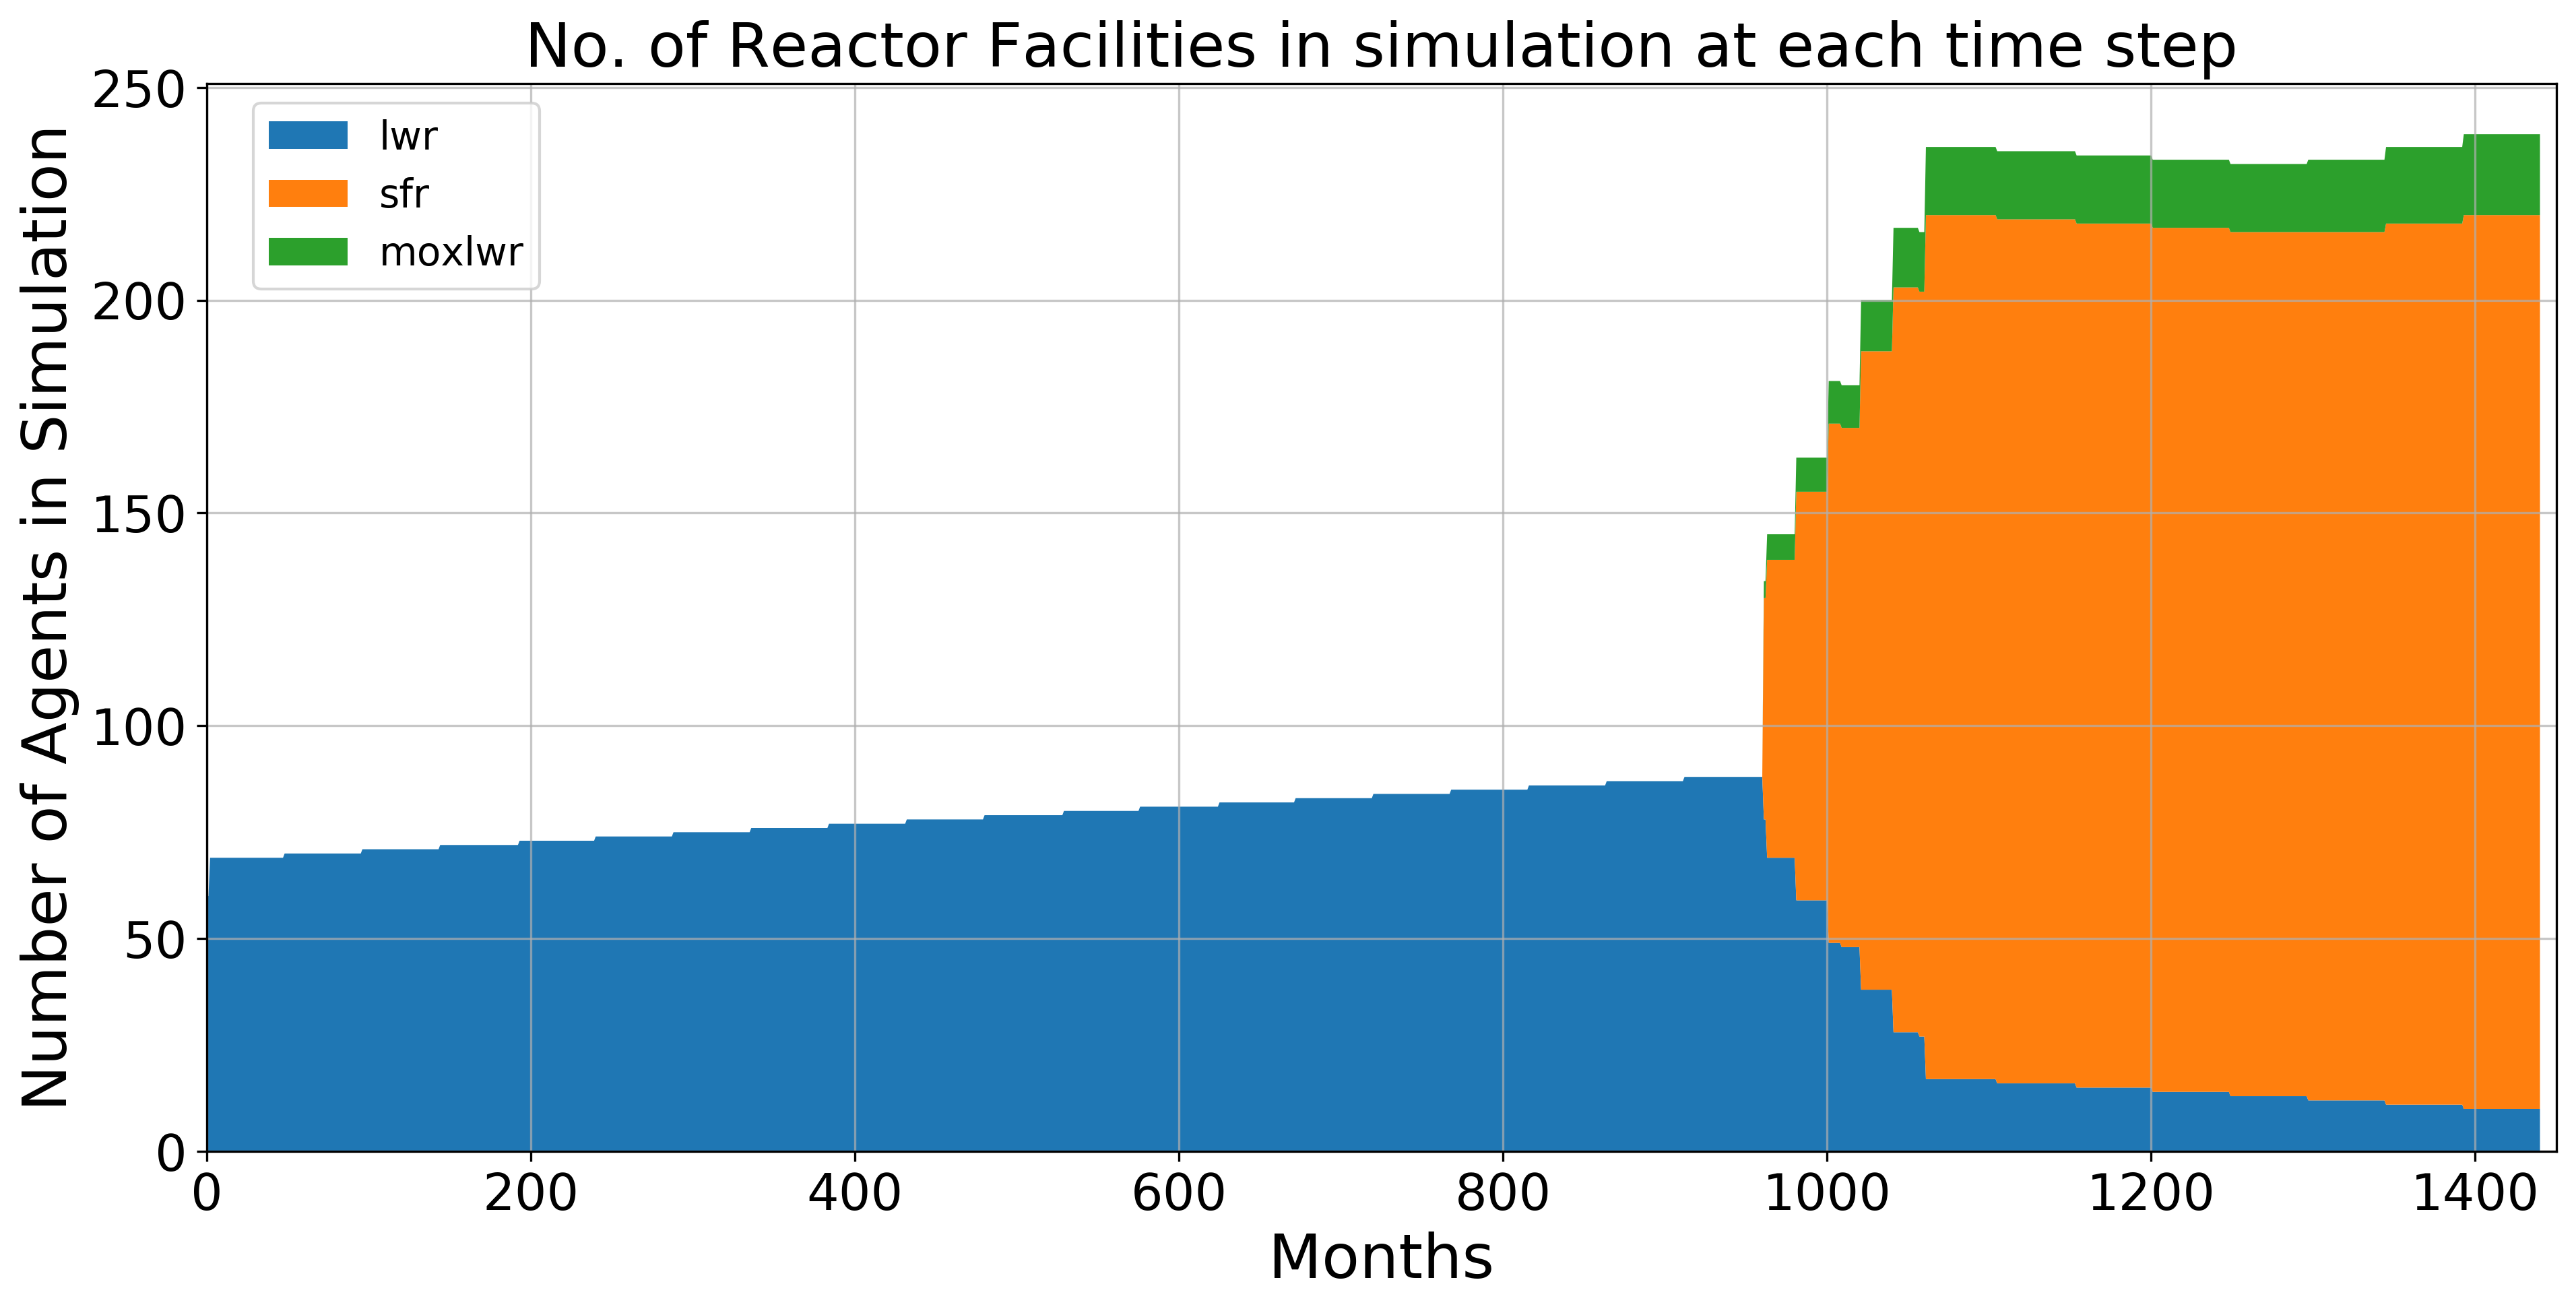
\includegraphics[width=\linewidth]{eg30-stack_reactor.png} 
		\caption{EG01-30: Reactor Deployment}
		\label{fig:30reactor}
	\end{subfigure}
	\vspace{1cm}
	\begin{subfigure}[t]{1.2\textwidth}
		\centering
		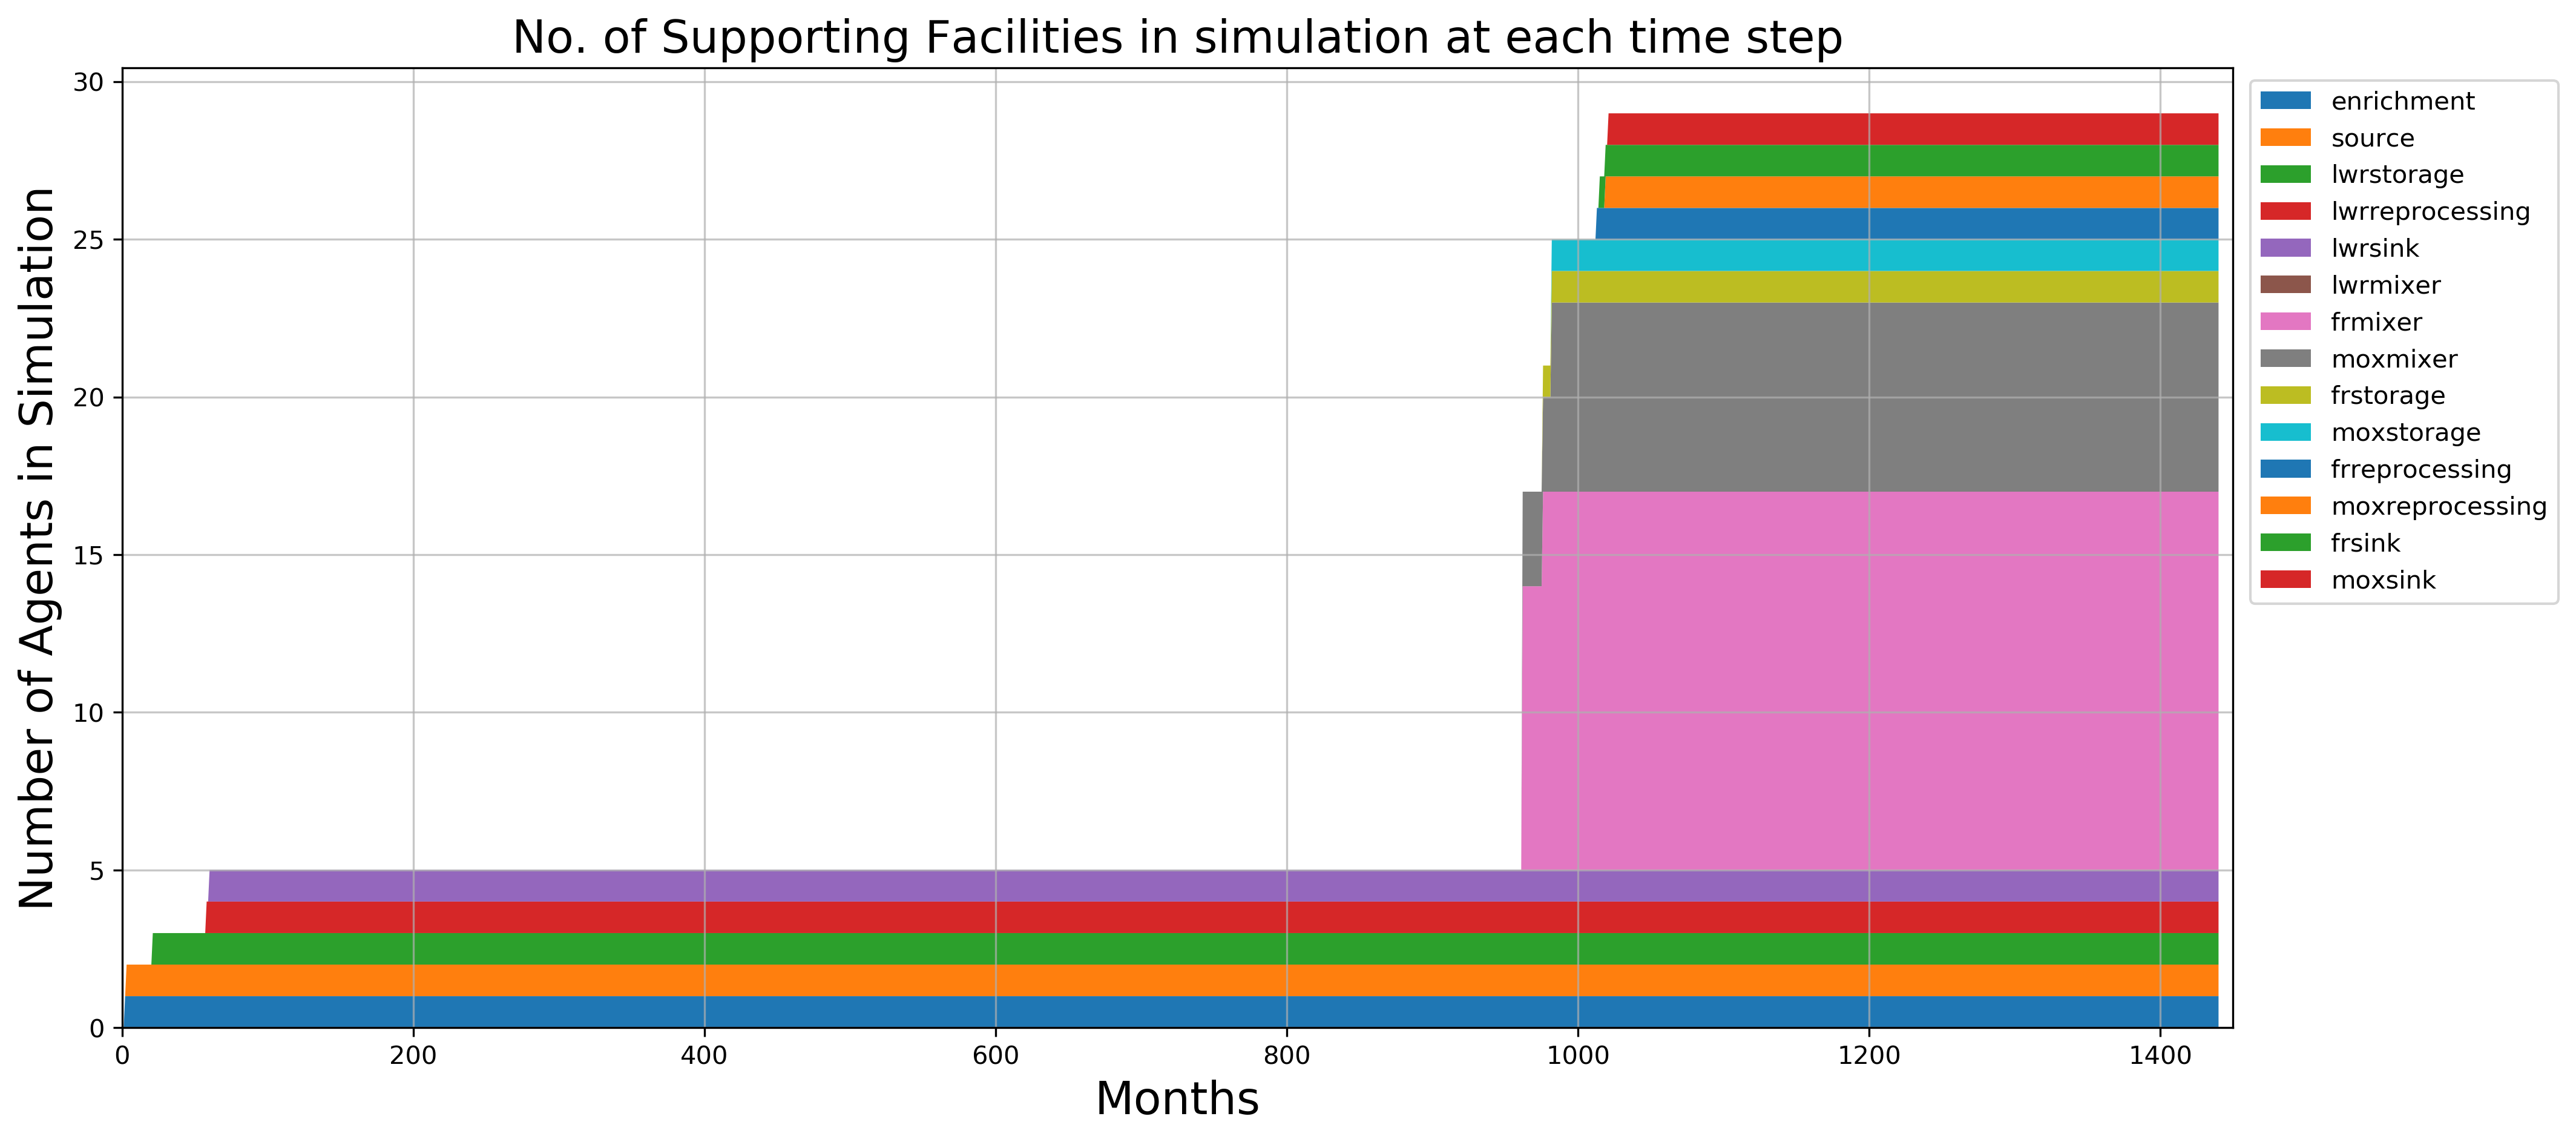
\includegraphics[width=\linewidth]{eg30-stack_support.png} 
		\caption{EG01-30: Supporting Facility Deployment}
		\label{fig:30support}
	\end{subfigure}
	\hfill
	\caption{Time dependent deployment of reactor and supporting facilities in 
	the EG01-30 linearly increasing power demand transition scenario. 
	\deploy automatically deploys reactor and supporting facilities 
	to setup a supply chain to meet linearly increasing power demand of $60000 + 250t/12$ MW
	during a transition from \glspl{LWR} to MOX LWRs and \glspl{SFR}. }
	\label{fig:30stack}
\end{figure}

\begin{table}[]
	\centering
        \caption{Undersupply/capacity of key commodities for the best performing EG01-EG23,24,29,30 transition scenarios.}
		\label{tab:all-power}
		\footnotesize
        \begin{tabular}{l|rrrr}
		\hline
		& \multicolumn{3}{c}{\textbf{Undersupplied Time Steps}} \\ \hline
		\textbf{Transition Scenario} & EG01-EG23 & 
		EG01-EG24 & EG01-EG29 & 
		EG01-EG30 \\ 
		\textbf{Power Demand [MW]} &60000&60000+250t/12&60000&60000+250t/12 \\
		\textbf{Prediction Method} &\texttt{POLY}&\texttt{FFT}&\texttt{POLY}& \texttt{FFT}\\
		\textbf{\shortstack{Power Buffer [MW]}} &0&6000&0&8000 \\ \hline
		\textbf{Commodities} \\ 
		Natural Uranium		    & 2 	& 3  &  1  & 1 \\ 
		\gls{LWR} Fuel     	    & 4 	& 6  &  1  & 2\\ 
		\gls{SFR} Fuel     	    &  0 	& 0  &  2  & 2\\ 
		\gls{MOX} \gls{LWR} Fuel &-&-&2&2 \\
		Power      				&  6 	& 7  &  4 &  5\\ 
		\gls{LWR} Spent Fuel	& 1 	& 1  & 1 & 1\\ 
		\gls{SFR} Spent Fuel     	    &  1 	& 1  &  1  & 1\\ 
		\gls{MOX} \gls{LWR} Spent Fuel &-&-&1&1 \\ \hline 
	\end{tabular}
\end{table}
